%================================================================
% SLO
%----------------------------------------------------------------
% datoteka: 	thesis_template.tex
%
% opis: 		predloga za pisanje diplomskega dela v formatu LaTeX na
% 				Univerza v Ljubljani, Fakulteti za računalništvo in informatiko
%
% pripravili: 	Matej Kristan, Zoran Bosnić, Andrej Čopar,
%			  	po začetni predlogi Gašperja Fijavža
%
% popravil: 	Domen Rački, Jaka Cikač, Matej Kristan
%
% verzija: 		30. september 2016 (dodan razširjeni povzetek)
%================================================================


%================================================================
% SLO: definiraj strukturo dokumenta
% ENG: define file structure
%================================================================
\documentclass[a4paper, 12pt]{book}

%================================================================
% SLO: Odkomentiraj "\SLOtrue " za izbiro slovenskega jezika
% ENG: Uncomment "\SLOfalse" to chose English languagge
%================================================================
\newif\ifSLO
% switch language

\SLOtrue % Enables Slovenian language
%\SLOfalse  % Enables English language

%================================================================
% SLO: vključi oblikovanje in pakete
% ENG: include design and packages
%================================================================
%----------------------------------------------------------------
% SLO: LaTeX paketi
% ENG: LateX packages
%----------------------------------------------------------------
% SLO: omogoča uporabo slovenskih (latinskih) črk kodiranih v formatu UTF-8
% ENG: enables the use of slovene (latin) caracters encoded in the UFT-8 format
\usepackage[utf8x]{inputenc}
%\inputencoding{utf8} 
% SLO: naloži, med drugim, slovenske delilne vzorce
% ENG: loads, among others, slovene dividing patterns
\usepackage[slovene,english]{babel} 
% SLO: poskrbi za postavitev strani
% ENG: takes care of the page layout
\usepackage{fancyhdr}
% SLO: za vlaganje slik različnih formatov
% ENG: for loading figures of different formats
\usepackage{graphicx}
\usepackage{caption}
\captionsetup[figure]{labelfont=bf} % SLO: napis "Slika #" v krepkem tisku
									% ENG: wirte "Figure #" caption in bold
\captionsetup[table]{labelfont=bf} % SLO: napis "Tabela #" v krepkem tisku
								   % ENG: wirte "Table #" caption in bold
% SLO: za pisanje psevdokode
% ENG: for writing pseudocode
\usepackage{algorithm}
\usepackage{algorithmic}
\floatname{algorithm}{\footnotesize Algorithm} % SLO: napis "Algoritem #" v krepkem tisku
											   % ENG: write "Algorithm #" caption in bold
% SLO: poveže reference slik/tabel in slike/tabele znotraj dokumenta
% ENG: links image/table references with the images/tables within the document
\usepackage{hyperref}
% SLO: pri kliku na referenco slike/tabele se postavi na vrh slike/tabele
% ENG: when clicking the image/table reference, position the focus on top of the image/table
\usepackage[all]{hypcap}
% SLO: omogoča, med drugim, definicjo in uporebo barve
% ENG: enables, among others, the definition and use of colors
\usepackage{xcolor}
%----------------------------------------------------------------
% SLO: dodatni paketi
% ENG: additional packages
%----------------------------------------------------------------
% SLO: omogoča večjo manipulacijo nad tabelami
% ENG: allows for greater manipulation of tables
\usepackage{booktabs}
% SLO: naloži dodatne simbole
% ENG: loads additional symbols
\usepackage{amssymb} 
% SLO: omogoča, med drugim, sklicevanje na formule z eqref
% ENG: enables, among others, equation referencing with eqref
\usepackage{amsmath}
% SLO: omogoča komentiranje večjega dela teksta
% ENG: enables the commenting of larger text parts
\usepackage{verbatim}
% SLO: omogoča rotacijo PDF strani v ležeč položaj
% ENG: enables the rotation of a PDF page to landscape
\usepackage{pdflscape}
% SLO: omogoča barvanje vrstic in stolpcev tabel
% ENG: enables coloring of table rows and columns
\usepackage{colortbl}
\usepackage{url}



%================================================================
% SLO: nastavitve dokumenta
% ENG: document properties
%================================================================
% SLO: prilagoditev robov za tisk
% ENG: margin adjustments for printing
\addtolength{\marginparwidth}{-20pt}
\addtolength{\oddsidemargin}{40pt}
\addtolength{\evensidemargin}{-40pt}
% SLO: razmik med vrsticami
% ENG: line spacing
\renewcommand{\baselinestretch}{1.3} 
% SLO: postavitev strani
% ENG: page layout
\renewcommand{\chaptermark}[1]{\markboth{\MakeUppercase{\thechapter.\ #1}}{}} 
\renewcommand{\sectionmark}[1]{\markright{\MakeUppercase{\thesection.\ #1}}} 
\renewcommand{\headrulewidth}{0.5pt} % Header rule
\renewcommand{\footrulewidth}{0pt} % Footer rule
%
\fancypagestyle{frontmatter}{%
	\fancyhf{} % Clear all headers and footers first
	\fancyhead[LE, RO]{\sl \thepage} 
	%\fancyhead[LO]{\sl \rightmark} 
	%\fancyhead[RE]{\sl \leftmark}
}
\fancypagestyle{mainmatter}{%
  	\fancyhf{} % Clear all headers and footers first
	\fancyhead[LE,RO]{\sl \thepage} 
	\fancyhead[LO]{\sl \rightmark} 
	\fancyhead[RE]{\sl \leftmark}
}
% SLO: font za ime avtorja
% ENG: font for author name
\newcommand{\authorfont}{\Large}
% SLO: font za naslov diplomskega dela
% ENG: font for thesis title
\newcommand{\titlefont}{\LARGE\bf}
% SLO: globina kazala
% ENG: content depth
\setcounter{tocdepth}{1}
% SLO: definiraj ukaz za prazno stran
% ENG: define the command for empty page
\newcommand{\clearemptydoublepage}{\newpage{\pagestyle{empty}\cleardoublepage}}

\newcommand{\BibTeX}{{\sc Bib}\TeX}


%----------------------------------------------------------------
% |||||||||||||||||||||| USTREZNO POPRAVI |||||||||||||||||||||||
% |||||||||||||||||||||| EDIT ACCORDINGLY |||||||||||||||||||||||
%----------------------------------------------------------------
\newcommand{\ttitle}{Oblikoskladenjsko označevanje slovenskega jezika z globokimi nevronskimi mrežami}
\newcommand{\ttitleEn}{Part of speech tagging of slovene language using deep neural networks}
\newcommand{\tsubject}{\ttitle}
\newcommand{\tsubjectEn}{\ttitleEn}
\newcommand{\tauthor}{Primož Belej}
\newcommand{\temail}{MAIL}
\newcommand{\myyear}{2018}
\newcommand{\tkeywords}{oblikoskladenjsko označevanje, globoko učenje, konvolucijske nevronske mreže}
\newcommand{\tkeywordsEn}{part-of-speech tagging, deep learning, convolutional neural network}
\newcommand{\mysupervisor}{prof.~dr.\ Marko Robnik Šikonja}
\newcommand{\mycosupervisor}{dr.\ Simon Krek}

% include formatted front pages

%----------------------------------------------------------------
% SLO: definiraj metapodatke za datoteko thesis_template.tex
% ENG: define metadata for the file thesis_template.tex
%----------------------------------------------------------------
%----------------------------------------------------------------
%	HYPERREF SETUP
% SLO: ustrezno popravi e-mail
% ENG: edit the e-mail accordingly
%----------------------------------------------------------------
\hypersetup{pdftitle={\ttitle}}
\hypersetup{pdfsubject=\ttitleEn}
\hypersetup{pdfauthor={\tauthor, \temail}}
%\hypersetup{pdfkeywords=\tkeywordsEn}

%----------------------------------------------------------------
% define medatata
% SLO: ustrezno popravi e-mail
% ENG: edit the e-mail accordingly
%----------------------------------------------------------------
\def\Title{\ttitle}
\def\Author{\tauthor, \temail}
\def\Subject{\ttitleEn}
\def\Keywords{\tkeywordsEn}
\def\Org{Univerza v Ljubljani, Fakulteta za računalništvo in informatiko}

%%%%%%%%%%%%%%%%%%%%%%%%%%%%%%%%%%%%%%%%
% \convertDate converts D:20080419103507+02'00' to 2008-04-19T10:35:07+02:00
%%%%%%%%%%%%%%%%%%%%%%%%%%%%%%%%%%%%%%%%
\def\convertDate{%
    \getYear
}

{\catcode`\D=12
 \gdef\getYear D:#1#2#3#4{\edef\xYear{#1#2#3#4}\getMonth}
}
\def\getMonth#1#2{\edef\xMonth{#1#2}\getDay}
\def\getDay#1#2{\edef\xDay{#1#2}\getHour}
\def\getHour#1#2{\edef\xHour{#1#2}\getMin}
\def\getMin#1#2{\edef\xMin{#1#2}\getSec}
\def\getSec#1#2{\edef\xSec{#1#2}\getTZh}
\def\getTZh +#1#2{\edef\xTZh{#1#2}\getTZm}
\def\getTZm '#1#2'{%
    \edef\xTZm{#1#2}%
    \edef\convDate{\xYear-\xMonth-\xDay T\xHour:\xMin:\xSec+\xTZh:\xTZm}%
}

\expandafter\convertDate\pdfcreationdate


%%%%%%%%%%%%%%%%%%%%%%%%%%%%%%%%%%%%%%%%
% get pdftex version string
%%%%%%%%%%%%%%%%%%%%%%%%%%%%%%%%%%%%%%%%
\newcount\countA
\countA=\pdftexversion
\advance \countA by -100
\def\pdftexVersionStr{pdfTeX-1.\the\countA.\pdftexrevision}

%%%%%%%%%%%%%%%%%%%%%%%%%%%%%%%%%%%%%%%%
% XMP data
%%%%%%%%%%%%%%%%%%%%%%%%%%%%%%%%%%%%%%%%
\usepackage{xmpincl}

%%%%%%%%%%%%%%%%%%%%%%%%%%%%%%%%%%%%%%%%
% pdfInfo
%%%%%%%%%%%%%%%%%%%%%%%%%%%%%%%%%%%%%%%%
\pdfinfo{%
    /Title    (\ttitle)
    /Author   (\tauthor, \temail)
    /Subject  (\ttitleEn)
    /Keywords (\tkeywordsEn)
    /ModDate  (\pdfcreationdate)
    /Trapped  /False
}

%================================================================
% SLO: razno
% ENG: other
%================================================================
% SLO: nastavitev sklicevanj
% ENG: hyper referencing setup
\definecolor{black}{rgb}{0,0,0}
\hypersetup{
	colorlinks = true,
	linkcolor = black,
	citecolor = black,
	urlcolor = black
}

%----------------------------------------------------------------
% SLO: dodaj poti do datotek s slikami, tabelami, ...
% ENG: add paths to files containing figures, tables, ...
%----------------------------------------------------------------
\graphicspath{
	{./figures/}
	{./tables/}
}
%----------------------------------------------------------------
% SLO: moji paketi
% ENG: my packages
%----------------------------------------------------------------
% ...
%----------------------------------------------------------------
% SLO: moji konstrukti
% ENG: my constructs
%----------------------------------------------------------------
\newtheorem{izrek}{Izrek}[chapter]
\newtheorem{trditev}{Trditev}[izrek]
\newenvironment{dokaz}{\emph{Dokaz.}\ }{\hspace{\fill}{$\Box$}}


%================================================================
% SLO: začetne strani magistrskega dela
% ENG: fist pages of the master's thesis
%================================================================
\begin{document}
% SLO: prepreči težave s številkami strani v kazalu
% ENG: prevents problems with the page numbers in the contents page
\renewcommand{\thepage}{}

%----------------------------------------------------------------
% Language-dependent formatting
%----------------------------------------------------------------
\ifSLO
    % SLO: definiraj slovensko besedo za kazalo
    \renewcommand{\contentsname}{Kazalo}

    % SLO: naslovnica (vstavi naslovnico (LaTeX kodo) iz datoteke pages/title.tex)
    \thispagestyle{empty}
	\begin{center}
        {\large\sc Univerza v Ljubljani\\Fakulteta za računalništvo in informatiko}
    	\vskip 10em
    	{\authorfont \tauthor \par}
    	{\titlefont \ttitle \par}
    {\vskip 2em \textsc{MAGISTRSKO DELO\\[2mm]
    MAGISTRSKI PROGRAM DRUGE STOPNJE\\RAČUNALNIŠTVO IN INFORMATIKA}\par}
    \vfill\null
    {\large \textsc{Mentor}: \mysupervisor \par}
   	{\large \textsc{Somentor}: \mycosupervisor \par}
    {\vskip 2em \large Ljubljana, \myyear \par}
\end{center} \clearemptydoublepage
    % SLO: avtorske pravice
    \thispagestyle{empty}
\vspace*{\fill}
{\noindent\footnotesize
{\sc Avtorske pravice}. Rezultati magistrskega dela so intelektualna lastnina avtorja in Fakultete za ra\-ču\-nal\-niš\-tvo in informatiko Univerze v Ljubljani. Za objavljanje ali izkoriščanje rezultatov ma\-gi\-str\-ske\-ga dela je potrebno pisno soglasje avtorja, Fakultete za ra\-ču\-nal\-niš\-tvo in informatiko ter mentorja\footnote{V dogovorju z mentorjem lahko kandidat magistrsko delo s pripadajočo izvorno kodo izda tudi pod drugo licenco, ki ponuja določen del pravic vsem: npr. Creative Commons, GNU GPL. V tem primeru na to mesto vstavite opis licence, na primer tekst~\cite{licence}.}.}
\begin{center}
{\footnotesize{\sc \copyright \myyear\ \tauthor}}
\end{center} \clearemptydoublepage
    % SLO: izjava o avtorstvu (ni več del vezane izdaje, ločena oddaja)
    % SLO: zahvala
    \thispagestyle{empty}

\begin{center}
{\Large \textbf{\sc Zahvala}}
\end{center}
\vspace{0.5cm}

{\it\noindent

% LKM
Zahvaljujem se prof. dr. Marku Robniku Šikonji za izvrstno mentorstvo, potrpežljivost, odzivnost in skrb za kvaliteto dela.

Somentorju, dr. Simonu Kreku, se zahvaljujem za temeljit strokovni pregled dela.

Hvala Tadeju Škvorcu, ki mi je omogočil delo na strežniku Laboratorija za kognitivno modeliranje.

Hvala materi in očetu za podporo in spodbudo med študijem. Hvala dragi sestri Neži za vse nasvete, ki so me usmerjali k cilju. Hvala sestri Barbari in bratu Petru.

Iz vsega srca se zahvaljujem svoji ženi Vesni, ki mi je ves čas stala ob strani, verjela vame in mi ni dovolila odnehati.

\vspace{0.5cm} \hfill \tauthor, \myyear
}
 \clearemptydoublepage
    % SLO: posvetilo
    %\thispagestyle{empty}\mbox{}{\vskip0.20\textheight}\mbox{}\hfill\begin{minipage}{0.55\textwidth}%

Vsem rožicam tega sveta.\\\\
\textit{''The only reason for time is so that everything doesn't happen at once.''}
\flushright --- Albert Einstein
\normalfont\end{minipage} \clearemptydoublepage
\else
    % ENG: title page (insert the title page (LaTeX code) from the file pages/title.tex)
    \thispagestyle{empty}
	\begin{center}
        {\large\sc University of Ljubljana\\Faculty of Computer and Information Science}
    	\vskip 10em
    	{\authorfont \tauthor \par}
    	{\titlefont \ttitleEn \par}
    {\vskip 2em \textsc{MASTER'S THESIS\\[2mm]
    THE 2nd CYCLE MASTER'S STUDY PROGRAMME\\COMPUTER AND INFORMATION SCIENCE}\par}
    \vfill\null
    {\large \textsc{Supervisor}: \mysupervisor \par}
   	{\large \textsc{Co-supervisor}:  \mycosupervisor \par}
    {\vskip 2em \large Ljubljana, \myyear \par}
\end{center}\thispagestyle{empty}
	\begin{center}
        {\large\sc University of Ljubljana\\Faculty of Computer and Information Science}
    	\vskip 10em
    	{\authorfont \tauthor \par}
    	{\titlefont \ttitleEn \par}
    {\vskip 2em \textsc{MASTER'S THESIS\\[2mm]
    THE 2nd CYCLE MASTER'S STUDY PROGRAMME\\COMPUTER AND INFORMATION SCIENCE}\par}
    \vfill\null
    {\large \textsc{Supervisor}: \mysupervisor \par}
   	{\large \textsc{Co-supervisor}:  \mycosupervisor \par}
    {\vskip 2em \large Ljubljana, \myyear \par}
\end{center}\include{title_page.tex}   \clearemptydoublepage
    % ENG: copyright
    \thispagestyle{empty}
\vspace*{\fill}
{\noindent\footnotesize
{\sc Copyright}. The results of this master's thesis are the intellectual property of the author and the Faculty of Computer and Information Science, University of Ljubljana. For the publication or exploitation of the master's thesis results, a written consent of the author, the Faculty of Computer and Information Science, and the supervisor is necessary.}
\begin{center}
{\footnotesize{\sc \copyright \myyear\ \tauthor}}
\end{center}  \clearemptydoublepage
    % ENG: declaration of authorship (not part of paper edition, turn in separately)
    % ENG: acknowledgements
    \thispagestyle{empty}

\begin{center}
{\Large \textbf{\sc Acknowledgments}}
\end{center}
\vspace{0.5cm}

{\it\noindent
Worth mentioning in the acknowledgment is everyone who contributed to your thesis.

\vspace{0.5cm} \hfill \tauthor, \myyear
} \clearemptydoublepage
    % ENG: dedication
    \thispagestyle{empty}\mbox{}{\vskip0.20\textheight}\mbox{}\hfill\begin{minipage}{0.55\textwidth}%

To all the flowers of this world.\\\\
\textit{''The only reason for time is so that everything doesn't happen at once.''}
\flushright --- Albert Einstein
\normalfont\end{minipage} \clearemptydoublepage
\fi

%----------------------------------------------------------------
% SLO: kazalo
% ENG: contents
%----------------------------------------------------------------
\begingroup
	\hypersetup{colorlinks=true,linkcolor=black}
	\def\thepage{}
	\tableofcontents{}
	\clearemptydoublepage
\endgroup


\ifSLO
    % SLO: seznam kratic
    \chapter*{Seznam uporabljenih kratic}

\begin{tabular}{l|l|l}
  {\bf kratica} & {\bf angleško} & {\bf slovensko} \\ \hline
  % after \\: \hline or \cline{col1-col2} \cline{col3-col4} ...
  {\bf CNN} & Convolutional neural network & Konvolucijska nevronska mreža \\
  {\bf CRF} & Conditional random fields & Pogojno naključna polja \\
  {\bf HMM} & Hidden Markov model & Skriti markovski model \\
  {\bf LSTM} & Long short-term memory & Nevronska mreža \\
             &  &  z dolgim kratkoročnim spominom \\
  {\bf MEMM} & Maximum entropy Markov model & Model maksimalne entropije \\
  {\bf RNN} & Recurrent neural network & Rekurentna nevronska mreža \\
\end{tabular}
 \clearemptydoublepage
    % SLO: glavne strani diplomskega dela
\else
    % ENG: list of acronmys
    \chapter*{List of used acronmys}

\begin{tabular}{l|l|l}
  {\bf acronym} & {\bf meaning}  \\ \hline
  % after \\: \hline or \cline{col1-col2} \cline{col3-col4} ...
  {\bf CA} & classification accuracy \\
  {\bf DBMS} & database management system \\
  {\bf SVM} & support vector machine \\
  ... & ... \\
\end{tabular} \clearemptydoublepage
\fi

\frontmatter
\pagestyle{frontmatter}
\setcounter{page}{1} %
\renewcommand{\thepage}{}       % preprecimo težave s številkami strani v kazalu


% include Slovenian abstract
%---------------------------------------------------------------
% SLO: slovenski povzetek
% ENG: slovenian abstract
%---------------------------------------------------------------
\selectlanguage{slovene} % Preklopi na slovenski jezik
\addcontentsline{toc}{chapter}{Povzetek}
\chapter*{Povzetek}

\noindent\textbf{Naslov:} \ttitle
\bigskip

V magistrskem delu se ukvarjamo z oblikoskladenjskim označevanjem slovenskega jezika. Pri tej nalogi s področja obdelave naravnega jezika povedim priredimo ustrezno zaporedje oznak, ki opisujejo oblikoskladenjske lastnosti besed. Za razliko od tipičnih pristopov, ki vhodne povedi obravnavajo na nivoju besed, naša rešitev obravnava vhodne povedi kot zaporedja znakov. Nalogo označevanja rešujemo s kombinacijo konvolucijskih in rekurentnih nevronskih mrež. Posebnost našega pristopa je tudi v sami naravi označevanja, saj ga ne obravnavamo kot problem večrazredne klasifikacije, temveč kot večznačno klasifikacijo, kjer primerom dodeljujemo oznake. Z namenom izboljšave rezultatov našo rešitev združimo v ansambel treh označevalnikov skupaj z dvema obstoječima označevalnikoma za slovenski jezik. Ob primerjavi naše rešitve z obstoječimi ugotovimo, da predlagana rešitev dosega najboljše rezultate pri reševanju zadanega problema.

\subsection*{Ključne besede}
\textit{\tkeywords}
\clearemptydoublepage

% include English abstract
 %---------------------------------------------------------------
% SLO: angleški povzetek
% ENG: english abstract
%---------------------------------------------------------------
\selectlanguage{english} % Preklopi na angleški jezik
\addcontentsline{toc}{chapter}{Abstract}
\chapter*{Abstract}

\noindent\textbf{Title:} \ttitleEn
\bigskip

This sample document presents an approach to typesetting your BSc thesis using \LaTeX. A proper abstract should contain around 100 words which makes this one way too short. A good abstract contains: (1) a short description of the tackled problem, (2) a short description of your approach to solving the problem, and (3) (the most successful) result or contribution in your thesis.

\subsection*{Keywords}
\textit{\tkeywordsEn}
\clearemptydoublepage

% Include extended abstract [Razširjeni povzetek v slovenščini-- le za dela pisana v angleščini]
\ifSLO
\else
  %  \cleardoublepage
    \let\oldthesection=\thesection %Special section numbering for this chapter - remember default one
    \let\oldthesubsection=\thesubsection
    \renewcommand{\thesection}{\Roman{section}} %Special section numbering for this chapter
    \renewcommand{\thesubsection}{\thesection.\Roman{subsection}}

    % set roman page numbering
    \pagenumbering{roman}
    % set slovene language
    \selectlanguage{slovene}
    % insert extended abstract
     \chapter{Razširjeni povzetek}
 
 To je primer razširjenega povzetka v slovenščini, ki je obvezen za naloge pisane v angleščini. Razširjeni povzetek mora vsebovati vse glavne elemente dela napisanega v angleščini skupaj s kratkim uvodom in povzetkom glavnih elementov metode, glavnih eksperimentalnih rezultatov in glavnih ugotovitev. Razširjeni povzetek naj bo strukturiran v podpoglavja (spodaj je naveden le okvirni primer in je nezavezujoč).
 Čez palec navadno razširjeni povzetek nanese okoli 10 odstotkov obsega celotnega dela. 
 
 \section{Kratek pregled sorodnih del}
 
 \section{Predlagana metoda}
 
 \section{Eksperimentalna evaluacija}
 
 \section{Sklep}
 
poljuben tekst  poljuben tekst  poljuben tekst  poljuben tekst  poljuben tekst  poljuben tekst  poljuben tekst  poljuben tekst  poljuben tekst  poljuben tekst  poljuben tekst  poljuben tekst  poljuben tekst  poljuben tekst  poljuben tekst  poljuben tekst  poljuben tekst  poljuben tekst  poljuben tekst  poljuben tekst  poljuben tekst  poljuben tekst  poljuben tekst  poljuben tekst  poljuben tekst  poljuben tekst  poljuben tekst  poljuben tekst  poljuben tekst  poljuben tekst  poljuben tekst  poljuben tekst  poljuben tekst  poljuben tekst  poljuben tekst  poljuben tekst  poljuben tekst  poljuben tekst  poljuben tekst  poljuben tekst  poljuben tekst  poljuben tekst  poljuben tekst  poljuben tekst  poljuben tekst  poljuben tekst  poljuben tekst  poljuben tekst  poljuben tekst  poljuben tekst  poljuben tekst  poljuben tekst  poljuben tekst  poljuben tekst  poljuben tekst  poljuben tekst  poljuben tekst  poljuben tekst  poljuben tekst  poljuben tekst  poljuben tekst  poljuben tekst  poljuben tekst  poljuben tekst  poljuben tekst  poljuben tekst  poljuben tekst  poljuben tekst  poljuben tekst  poljuben tekst  poljuben tekst  poljuben tekst  poljuben tekst  poljuben tekst  poljuben tekst  poljuben tekst  poljuben tekst  poljuben tekst  poljuben tekst  poljuben tekst  poljuben tekst  poljuben tekst  poljuben tekst  poljuben tekst  poljuben tekst  poljuben tekst  poljuben tekst  poljuben tekst  poljuben tekst  poljuben tekst 


    \let\thesection=\oldthesection % Restore default section numbering
    \let\thesubsection=\oldthesubsection
\fi

%----------------------------------------------------------------
% SLO: Preklopi izbrani jezik
% ENG: Switch to chosen language
%----------------------------------------------------------------
\ifSLO
    \selectlanguage{slovene} % Preklopi na slovenski jezik
\else
    \selectlanguage{english}  % Switch to english language
\fi

% SLO: vklopi številčenje poglavji, ponastavi številčenje strani in uporabi arabske številkami za številčenje strani
% ENG: turns on chapter numbering, resets page numbering and uses arabic numerals for page numbers
\mainmatter
\pagestyle{mainmatter}
\setcounter{page}{1}
\pagestyle{fancy}


%================================================================
% ENG: main pages of the thesis
%================================pic2================================
%----------------------------------------------------------------
% Poglavje (Chapter) 1
%----------------------------------------------------------------
\chapter{Uvod}
\label{ch:uvod}

% Motivacija

%% kaj je POSTagging
Oblikoskladenjsko označevanje je naloga s področja obdelave naravnega jezika. Cilj te naloge je za vhodne povedi v naravnem jeziku poiskati ustrezno zaporedje oblikoskladenjskih oznak. Oblikoskladenjske oznake vsebujejo informacijo o besedni vrsti in dodatnih morfoloških lastnostih besed.

%% zakaj POSTagging
Ta naloga je pomemben del predpriprave besedil na nadaljnje naloge s področja strojne obdelave naravnega jezika. S pomočjo oznak se lahko računalniški algoritmi naučijo natančneje prevajati besedila, povzemati njihovo vsebino in opravljati druge naloge, pri katerih je koristno poznavanje morfologije besed.

%% Kako se lotiti POSTagginga (splošno)
Računskega oblikoskladenjskega označevanja se lotevamo predvsem z algoritmi strojnega učenja. Za označevanje morfološko bogatih jezikov, med katere prištevamo tudi slovenščino, so se za učinkovite izkazali označevalniki temelječi na globokih nevronskih mrežah. Na globokih nevronskih mrežah temelji tudi naš označevalnik, ki ga bomo predstavili v nadaljevanju.

% Napoved vsebine po poglavjih

% 2. poglavje - Oblikoskladenjsko označevanje
V poglavju REF predstavimo oblikoskladenjsko označevanje in algoritmične pristope k oblikoskladenjskem označevanju. Opišemo probleme, ki se pojavljajo pri tej nalogi, načine reševanja teh problemov in posebnosti pri označevanju besedil v slovenskem jeziku. V tem poglavju naredimo tudi pregled obstoječih označevalnikov za slovenski jezik.

% 3. poglavje - Globoke nevronske mreže za besedila
Uporabo nevronskih mrež pri obdelavi besedil opišemo v poglavju REF. Predstavimo arhitekture nevronskih mrež, ki se uporabljajo pri obdelavi besedil. Opišemo tudi prispevke s tega področja, ki so vplivala na zasnovo naše rešitve.

% 4. poglavje - Arhitektura rešitve
Sledi poglavje REF z opisom naše rešitve. Na tem mestu opišemo podatke s katerimi delamo, pripravo podatkov na modeliranje in zgradbo našega modela. Pri zgradbi modela opišemo arhitekturo posameznih nevronskih mrež, ki sestavljajo našo rešitev.

% 5. poglavje - Evalvacija
Naš nevronski označevalnik ovrednotimo v poglavju REF. V tem poglavju opišemo postopek ocenjevanja napovedi našega označevalnika in naredimo primerjavo našega označevalnika s sorodnimi.

% 6. poglavje - Zaključki
V sklepnem poglavju izpostavimo glavne prispevke našega dela in komentiramo rezultate primerjave označevalnikov. Navedemo tudi razmisleke o možnih izboljšavah naše rešitve.


%----------------------------------------------------------------
% Poglavje (Chapter) 2
%----------------------------------------------------------------
\chapter{Oblikoskladenjsko označevanje}
\label{ch:pos}

% * kaj je to pos tagging
V uvodu smo povedali, da pri oblikoskladenjskem označevanju pripisujemo besedam oblikoskladenjske oznake in da te oznake vsebujejo informacijo o besedni vrsti in pripadajočih morfoloških in oblikovnih lastnostih.

% * zakaj ga rabimo
Besedilo je po naravi nestrukturirana oblika podatkov, zaradi česar je iz njega težko računsko izpeljevati sklepe o pomenu. Oblikoskladenjske oznake vnesejo v besedilo strukturo in tako olajšajo odkrivanje pomena in nadaljnjo delo, ki zahteva semantično razumevanje.

Oblikoskladenjske oznake se uporabljajo kot dodatne značilke pri algoritmičnem reševanju nalog kot sta (REF jurafsky ch8):
\begin{description}
    \item[Določanje imenskih entitet] Poznavanje oblikoskladenjskih oznak olajša določanje entitet (osebe, organizacije, ...). Imenske entitete se uporabljajo pri luščenju informacij iz besedila.
    \item[Prepoznava govora in tvorjenje govora] Za pravilno naglaševanje besed in poudarke pri izgovorjavi povedi.
\end{description}

\begin{table}
\caption{Primer označene povedi: "To bi bila pravična vojna."}
    \begin{center}
        \begin{tabular}{l l l}
\hline
Beseda & Oznaka & Pomen oznake \\ \hline
To & Zk-sei & Zaimek, kazalni, srednji spol, ednina, imenovalnik \\
bi & Gp-g & Glagol, pomožni, pogojnik \\
bila & Gp-d-ez & Glagol, pomožni, deležnik, ednina, ženski spol \\
pravična & Ppnzei & Pridevnik, splošni, nedoločena stopnja, ženski spol, ednina, imenovalnik \\
vojna & Sozei & Samostalnik, občno ime, ženski spol, ednina, imenovalnik \\
. & Z  & Ločilo \\
\hline
        \end{tabular}
    \end{center}
\label{tbl:oznacenapoved}
\end{table}

V tabeli ~\ref{tbl:oznacenapoved} vidimo primer označene povedi skupaj z razlago posameznih oznak. Primer je vzet iz jezikovnega korpusa ssj500k(\cite{ssj500kv2}), v katerem so uporabljene oblikoskladenjske oznake iz nabora MULTEXT-East.

% V tem poglavju hočem povedati:
% * kako se tega lotevamo
% * kakšni so klasični algoritmični pristopi s strojnim učenjem
% * kakšne težave se pojavljajo pri označevanju slovenskega jezika
% * kaj je to označevalnik Obeliks, kako deluje in kakšne rezultate dosega
% * kaj je označevalnik Reldi, kako deluje in kakšne rezultate dosega

\section{Algoritmične rešitve}
\label{sec:pos:alg}
Za določanja oblikoskladenjskih oznak ne zadostujejo enolične preslikave iz besed v oznake, saj za en zapis besede običajno velja mnogo različnih oznak. Za doseganje visoke točnosti oznak, se uporablja predvsem algoritme strojnega učenja.

V tem podpoglavju bomo predstavili pogoste pristope k označevanju z uporabo strojnega učenja. Pristop z nevronskimi mrežami, ki smo ga uporabili v tem diplomskem delu, bomo podrobneje predstavili v naslednjih dveh poglavjih (~\ref{ch:nn}, ~\ref{ch:arhitektura}).

\subsection*{Skriti markovski modeli}
% HMM na kratko
Skriti markovski modeli (Hidden Markov models, HMM) so sekvenčni modeli. Sekvenčni model vsakemu elementu zaporedja dodeli oznako ali razred. Sekvenčni model torej dela preslikave iz zaporedja opažanj v zaporedje oznak, kar tudi ustreza zahtevam oblikoskladenjskega označevanja: poved je zaporedje opažanj, oznake besed v povedi pa so zaporedje razredov.

% HMM delovanje
HMM deluje tako, da izračuna verjetnostno porazdelitev za vsa možna zaporedja oznak pri nekem zaporedju opažanj in izbere najverjetnejše zaporedje. Gre za nadgradnjo Markovskih verig, modelov s katerimi opisujemo verjetnosti zaporedja slučajnih spremenljivk, ki imajo za zalogo vrednosti množico stanj. Markovske verige niso primerne za označevanje, ker opisujejo samo vidna stanja, ne pa tudi skritih stanj. V primeru oblikoskladenjskega označevanja so vidna stanja besede, skrita stanja pa oznake. Označevanje s skritim markovskim modelom je prikazano na skici (~\ref{fig:hmm}).

Skriti markovski modeli prvega reda imajo dve predpostavki:
\begin{description}
	\item[Markovska predpostavka] Neko skrito stanje je odvisno le od prvega predhodnega skritega stanja, ne pa tudi od drugih predhodnih skritih stanj v zaporedju.
	$$ P(q_i|q_1...q_{i-1}) = P(q_i|q_{i-1}) $$
	\item[Neodvisnost opažanj] Neko opažanje je odvisno le od skritega stanja, ki je povzročilo to opažanje, ne pa tudi od drugih opažanj ali skritih stanj.
	$$ P(o_i|q_1...q_i,...,q_T,o_1,...,o_i,...,o_T)=P(o_i|q_i) $$
\end{description}

% HMM shema
\begin{figure}
\centering
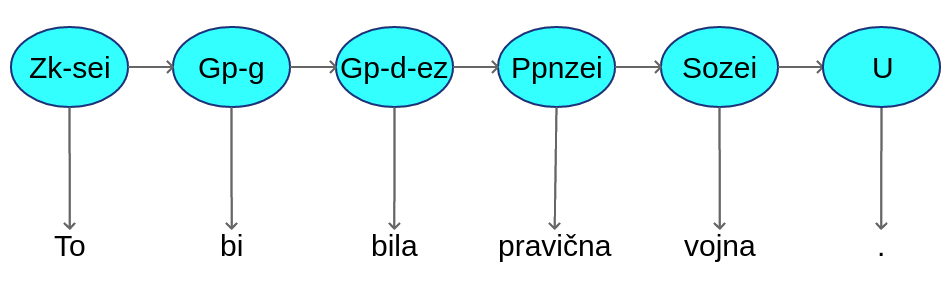
\includegraphics[width=1.0\textwidth]{hmm.png}
\caption{Označevalnik implementiran s skritim markovskim modelom. Ker gre za osnovni model prvega reda je oznaka odvisna le od predhodne oznake.}
\label{fig:hmm}
\end{figure}

Postopek prirejanja zaporedja oznak zaporedju opažanj imenujemo dekodiranje. Pri postopku dekodiranja iščemo najverjetnejše zaporedje skritih stanj. Za dekodiranje uporabljamo Viterbijev algoritem, ki s pomočjo dinamičnega programiranja zgradi matriko verjetnosti, s stolpcem za vsako opaženo stanje in vrstico za vsako možno oznako.

% HMM prednosti
% HMM slabosti
Označevalniki osnovani na skritih markovskih modelih v praksi uporabljajo izboljšave osnovnega markovskega modela prvega reda. Prva takšna izboljšava je razširitev kontekstnega okna. Pri računanju verjetnosti za neko oznako pri prejšnjih dveh oznakah dobimo trigramski model. Takšna razširitev navadno prinese izboljšave k točnosti označevanja, a se hkrati poveča tudi kompleksnost dekodiranja.

\begin{description}
	\item[Bigramski model] $ P(t_1^n) \approx \prod_{i=1}^{n}P(t_i|t_{i-1}) $
	\item[Trigramski model] $ P(t_1^n) \approx \prod_{i=1}^{n}P(t_i|t_{i-1}, t_{i-2}) $
\end{description}

Pogosta težava se pojavi pri neznanih besedah. Neznane besede so takšne, ki se niso pojavile v učni množici in jih algoritem še ni videl. To težavo rešujemo z obravnavanjem delov besed kot so pogoste končnice, začetki besed in velike začetnice.

S takšnimi izboljšavami so lahko skriti markovski modeli primerno orodje za označevanje Brants(2000) REF poroča o 96.7\% točnosti označevanja, kar je primerljivo z modeli maksimalne entropije in nevronskimi označevalniki.


\subsection*{Modeli maksimalne entropije} \label{postagging:mme}
Pri markovskih modelih maksimalne entropije (maximum entropy Markov models, MEMM) gre za model logistične regresije uporabljen na poseben način. Logistična regresija je klasifikacijski algoritem, ki pa ni sekvenčen in je tako sam po sebi neprimeren za označevanje zaporedij. Če uporabimo logistično regresijo na zaporednih besedah v povedi in uporabimo poleg ostalih vhodnih parametrov še napoved prejšnjega modela, dobimo model MEMM.

% shema memm
\begin{figure}
\centering
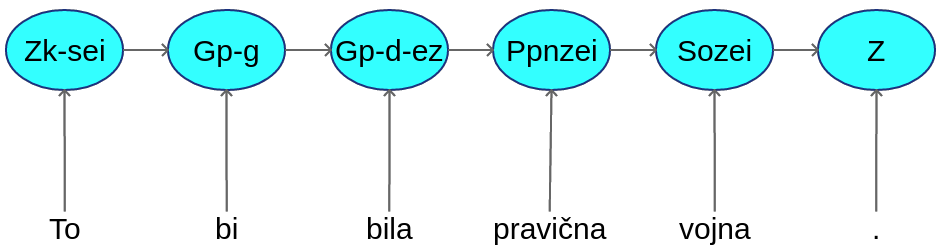
\includegraphics[width=1.0\textwidth]{memm.png}
\caption{Označevalnik implementiran z modelom maksimalne entropije.}
\label{fig:memm}
\end{figure}

Z uporabo takšnih modelov, lahko preprosteje vključujemo poljubne značilke, kar je pri generativnih modelih, kot je HMM, težje. Pri implementaciji označevalnikov, z uporabo modelov maksimalne entropije vključujemo večje število značilk. Te značilke so običajno sosednje besede in oznake v oknih različnih širin, predpona in končnica besede, prisotnost velikih začetnic, številk, simbolov in podobno.

Najpreprostejši način dekodiranja modelov maksimalne entropije je z uporabo požrešnega dekodirnega algoritma. Ta pristop deluje tako, da s klasifikatorjem napovemo oznake vseh besed iz ene smeri v drugo in pri tem napovedi oznak klasifikatorja posredujemo naslednjim stopnjam. Takšen pristop je hiter, a ponavadi njegova točnost ni zadostna, saj so napovedi oznak na vsakem koraku dokončne in jih klasifikator v kasnejših  korakih ne more popraviti. Ustreznejši postopek dekodiranja je z uporabo Viterbijevega algoritma, kot pri skritih markovskih modelih. Na skici modela (~\ref{fig:memm}) opazimo, da je oznaka odvisna od predhodne oznake in trenutne besede.


\subsection*{Dvosmerno označevanje}
Pomanjkljivost modelov maksimalne entropije in skritih markovskih modelov pri označevanju besedil je v tem, da označuje le v smeri od začetka do konca povedi. To je težava, ker so besede in njihove oznake med sabo odvisne v obeh smereh. V izogib negativnim posledicam označevanja v eno smer se uporabljajo različni pristopi:
\begin{itemize}
	\item Vsak sekvenčni model lahko spremenimo v dvosmerni model z uporabo večkratnih prehodov. Ob prvem prehodu model uporablja samo oznake že označenih besed levo od trenutno označevane besede, v drugem prehodu pa lahko uporablja tudi oznake besed, ki se nahajajo desno od trenutne in so bile označene v prejšnjem prehodu.
	\item Pristop podoben večkratnim prehodom sta dva prehoda, vsak v svoji smeri. Ker imamo tu opravka z verjetnostnimi modeli lahko izberemo oznake, ki jima model pripiše višje verjetnosti.
	\item Označevalnik Stanford Tagger CITE (Toutanova et al., 2003). uporablja dvosmerno različico modela maksimalne entropije, ki se imenuje ciklično odvisnostno omrežje (cyclic dependency network	
\end{itemize} 


\subsection*{Pogojno verjetnostna polja}
\label{pos:alg:crf}
Modeli pogojno verjetnostnih polj (Conditional random fields, CRF) so neusmerjeni verjetnostni grafični modeli in že v svoji osnovi odpravljajo težavo enosmernega označevanja REF. Ti modeli dosegajo najboljše rezultate pri različnih nalogah označevanja zaporedij.

Modeli CRF normalizirajo verjetnosti za celotno zaporedje oznak in ne lokalno, kot modeli MEMM. Prednost tega je, da modeli CRF niso pristranski k nekaterim oznakam. Modeli CRF so kompleksnejši od modelov HMM in MEMM, zato njihovo učenje traja dlje časa.

%skica
\begin{figure}
\centering
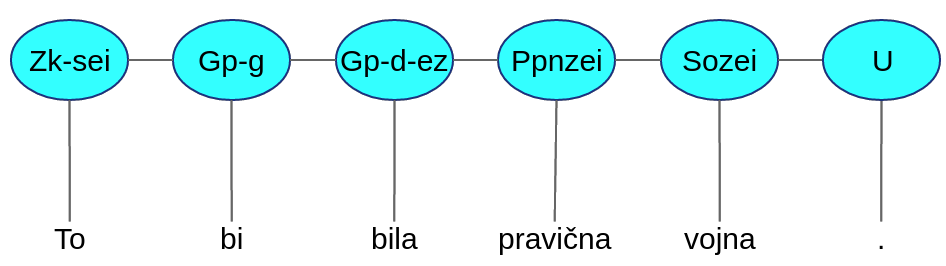
\includegraphics[width=1.0\textwidth]{crf.png}
\caption{Označevalnik implementiran s pogojno verjetnostnim poljem.}
\end{figure}

\section{Oblikoskladenjsko označevanje slovenščine}
\label{sec:pos:slo}
Težavnost opisanega problema se med različnimi naravnimi jeziki razlikuje. Na težavnost pomembno vpliva število možnih oznak v jeziku. Teh v slovenskem jeziku poznamo 1900 (REF MULTEXT-East V5), medtem ko nabori oznak za angleški jezik navadno vsebujejo med 45 in 100 različnih oznak (REF). Razlog za veliko število možnih oznak v slovenskem jeziku je veliko število različnih oblik v katerih zapisujemo besede. Dve besedi z isto osnovno obliko, z eno različno lastnostjo imata običajno v slovenščini različna zapisa.

Jezikom, pri katerih se pojavljajo omenjene lastnosti, pravimo morfološko bogati jeziki (REF jurafsky). Med te jezike, poleg slovenščine, uvrščamo jezike kot so turščina, madžarščina in češčina.

Oblikoskladenjske oznake v morfološko bogatih jezikih nosijo več informacij kot oznake v jezikih kakršen je angleški. V morfološko bogatih jezikih poznamo koncept sklona, časa, števila, osebe in drugih lastnosti, ki so značilne samo za določene besedne vrste. Oblikoskladenjske oznake v takšnih jezikih so zaporedja morfoloških oznak in ne enotne, primitivne oznake.

% Specifikacije JOS
V okviru pričujočega magistrskega dela smo uporabljali oblikoskladenjske oznake, določene v specifikaciji MULTEXT-East V5. Ta specifikacija uporablja trinajst besednih vrst: samostalnik, glagol, pridevnik, prislov, zaimek, števnik, predlog, veznik, členek, medmet, okrajšava, neuvrščeno in ločilo.

V tabeli ~\ref{tbl:besednevrste} so za slovenščino po MULTEXT-East V5 navedene besedne vrste, število lastnosti za posamezno besedno vrstno in število vseh veljavnih kombinacij lastnosti.

\begin{table}
\caption{Besedne vrste po specifikaciji MULTEXT-East V5.}
    \begin{center}
        \begin{tabular}{l l l}
        \hline
Besedna vrsta & Število lastnosti & Število možnih kombinacij \\ \hline
Samostalnik & 5 & 104 \\
Glagol & 7 & 156 \\
Pridevnik & 6 & 279 \\
Prislov & 2 & 4 \\
Zaimek & 8 & 1122 \\
Števnik & 6 & 215 \\
Predlog & 1 & 6 \\
Veznik & 1 & 2 \\
Členek & 0 & 1 \\
Medmet & 0 & 1 \\
Okrajšava & 0 & 1 \\
Neuvrščeno & 1 & 8 \\
Ločilo & 0 & 1 \\ \hline
        \end{tabular}
    \end{center}
\label{tbl:besednevrste}
\end{table}

% primer prostega besednega reda in zakaj je to slabo za HMM
Lastnost slovenščine, ki dodatno vpliva na težavnost označevanja je prost besedni red. Zaradi te lastnosti se lahko besede pojavljajo na različnih mestih v povedi, ne da bi spremenile pomen povedi. Povedi v spodnjem primeru so sestavljene iz istih besed, spremenili smo le njihov vrstni red.

\begin{itemize}
\item Vesna na vrtu nabira rože.
\item Na vrtu Vesna nabira rože.
\item Rože na vrtu nabira Vesna.
\end{itemize}

Vse povedi so sintaktično pravilne in nosijo isti pomen. Razlika je le v poudarku. Prost vrstni red besed uvede dodatno težavnost za jezikovne modele, saj je zaradi te lastnosti težje prepoznati vzorce, ki se pojavljajo v jeziku.

\section{Obstoječe rešitve}
\label{sec:pos:solutions}
Najuspešnejši obstoječi izvedbi označevalnika za slovenski jezik sta označevalnika Obeliks in Reldi. Temeljita na algoritmih strojnega učenja, ki smo jih opisali v podpoglavju ~\ref{sec:pos:alg}.

\subsection*{Grčar, Krek, Dobrovoljc (2012)\cite{Grcar2012}}
V okviru projekta Sporazumevanje v slovenskem jeziku CITE je skupina raziskovalcev razvila orodje imenovano Obeliks. Obeliks ni samo oblikoskladenjski označevalnik. Vključuje tudi orodja za segmentacijo, tokenizacijo in lematizacijo besedila. Segmentacija poskrbi za razdelitev vhodnega besedila na enote za označevanje, ki so običajno povedi. Tokenizacija poišče pojavnice. Pojavnice so največkrat ločila in besede. Lematizacija določa besedam njihovo osnovno obliko.

Za označevanje besed so uporabili model maksimalne entropije (~\ref{postagging:mme}. Model so naučili na jezikovnem korpusu ssj500k \cite{ssj500kv13}. Poleg tipičnih značilk, kot so sosednje besede in oznake prejšnjih besed, so uporabili še potencialne oznake iz drevesa končnic, zgrajenega na podlagi učnega korpusa. Pri napovedovanju besedne vrste je označevalnik dosegel 98,3 \% točnost, celotne oznake pa je določal z 91,34 \% točnostjo.

\begin{figure}
\centering
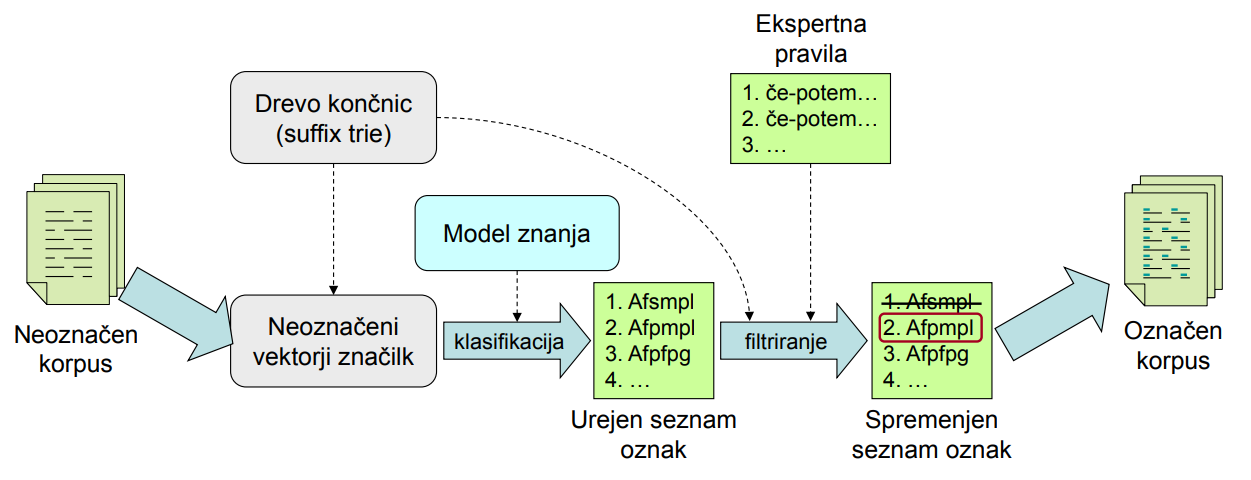
\includegraphics[width=1.0\textwidth]{obeliks.png}
\caption{Shema delovanja orodja Obeliks in njegovih komponent.}
\end{figure}

\subsection*{Ljubešić, Erjavec (2016)\cite{Ljubesic2016}}
Avtorji tega dela so razvili nov označevalnik, osnovan na modelu pogojno naključnih polj (~\ref{pos:alg:crf}). Njihov označevalnik se imenuje Reldi. Za osnovo so uporabili označevalnik Obeliks. Tako kot označevalnik Obeliks, tudi Reldi za dodatne značilke uporablja drevo končnic. Svoj označevalnik so posebej optimizirali za označevanje neznanih in delno neznanih besed. Označevanje neznanih besed je del arhitekture označevalnika in tega ne rešuje dodaten proces, kot je bilo običajno pri označevalnikih za morfološko bogate jezike.

Poročajo o 98,94\% točnosti pri napovedovanju besedne vrste, za celotne oznake pa 94,27\%. 

%----------------------------------------------------------------
% Poglavje (Chapter) 3
%----------------------------------------------------------------
\chapter{Globoke nevronske mreže za besedila}
\label{ch:nn}
V prejšnjem poglavju smo predstavili nekatere algoritmične pristope k oblikoskladenjskem označevanju. Za reševanje te naloge, pa tudi drugih s področja obdelave naravnega jezika, postajajo v zadnjih letih vedno pogostejši pristopi z uporabo nevronskih mrež.

V tem poglavju bomo predstavili vrste nevronskih mrež, ki se pogosto uporabljajo na področju obdelave naravnega jezika. Te vrste smo uporabili tudi mi pri implementaciji naše rešitve. Na koncu poglavja predstavimo tudi prispevke s tega področja, ki so vplivali na našo rešitev.

\section{Konvolucijske nevronske mreže}
\label{sec:nn:cnn}
Konvolucijske nevronske mreže so posebna vrsta nevronskih mrež, namenjene obdelavi podatkov razporejenih v vnaprej znano strukturo. Slike, kjer se konvolucijske nevronske mreže pogosto uporabljajo, imajo slikovne točke razporejene v dvodimenzionalno strukturo. Besedila navadno opisujemo z enodimenzionalo strukturo, saj imamo opravka z enodimenzionalnimi zaporedji besed ali znakov. Konvolucijske nevronske mreže se imenujejo po matematični operaciji konvoluciji, ki jo uporabljajo vsaj na enem nivoju, namesto običajnega matričnega množenja.

\subsection*{Konvolucija}
Konvolucijo opisuje spodnja enačba (\ref{eq:cnn:conv}).V kontekstu, ko je $t$ časovna komponenta, lahko konvolucijo opišemo kot uteženo povprečje funkcije $x$, v trenutku $t$, utež pa dobimo iz funkcije $w(-a)$, z zamikom $t$. S spremembo parametra $t$ se spreminja tudi vrednost uteži $w(t-a)$.

\begin{equation}
\label{eq:cnn:conv}
s(t) = \int x(a)w(t-a)da
\end{equation}

Čeprav smo vhodni parameter poimenovali $t$, ni potrebno, da le ta opisuje čas. Čas bi bil primeren parameter pri modeliranju časovnih vrst, pri besedilih pa je to položaj v besedilu.

Operacijo konvolucije običajno zapisujemo s simbolom $*$ in tako lahko zgornjo enačbo zapišemo kot:
\begin{equation}
s(t) = (x * w)(t)
\end{equation}

Zgornja definicija konvolucije predvideva, da je časovna spremenljivka $t$ zvezna, kar pa ne drži, kadar imamo opravka s podatki v nevronskih mrežah, saj podatki prihajajo v diskretnih enotah, kot so slikovne točke, besede, ali črke. Tudi pri obdelavi časovnih vrst imamo v resnici opravka z diskretnimi podatki. Za modeliranje z nevronskimi mrežami je ustreznejša definicija, ki obravnava spremenljivko $t$ kot diskretno:
\begin{equation}
s(t)=(x*w)(t) =  \sum_{a=-\infty }^{\infty } x(a)w(t-a)
\end{equation}

V kontekstu nevronskih mrež, pravimo argumentu $x(a)$ vhod, drugemu argumentu $w(t-a)$ pa jedro. V praksi so podatki na vhodu običajno v obliki večdimenzionalnih polj, ki jih imenujemo tenzorji. Jedro je prav tako tenzor parametrov, ki jih nastavi algoritem strojnega učenja.

Kadar se konvolucija uporablja na dvo ali večdimenzionalnih podatkih, uporabimo razširjeno definicijo konvolucije, ki deluje na več oseh. Naslednja enačba (\ref{eq:cnn:2d}) definira konvolucijo na dveh oseh. Vhod I in jedro K sta dvodimenzionalni polji.

\begin{equation}
\label{eq:cnn:2d}
S(i, j)=(I*K)(i,j) =  \sum_{m}\sum_{n}I(m,n)K(i-m,j-n)
\end{equation}

\subsection*{Lastnosti konvolucijskih nevronskih mrež}

Prehodi med sloji v nevronskih mrežah so običajno predstavljeni z matričnim množenjem. Elementi matrike so uteži povezav med posameznimi vhodnimi in izhodnimi enotami. V takšnih gosto povezanih nevronskih mrežah je vsak izhod povezan z vsakim izhodom. Konvolucijske nevronske mreže se razlikujejo od običajnega pristopa v tem, da imajo redkejše povezave. Ta lastnost izhaja iz tega, da je jedro konvolucije največkrat manjše od vhoda. Takšen pristop ima pri določenih nalogah številne prednosti pred klasičnim:
\begin{itemize}
\item Manjša prostorska zahtevnost, ki izvira iz tega, da ni potrebno shranjevati uteži povezav med vsemi vhodi in izhodi.
\item Manjša računska zahtevnost učenja. Za izračun vrednosti na izhodih je potrebnih manj računskih operacij.
\item Več različnih funkcij modela si lahko deli isti parameter. Pri običajnih nevronskih mrežah se vsak parameter iz matrike uteži uporabi natanko enkrat, pri konvolucijskih nevronskih mrežah pa se vsak element jedra uporabi na vsakem elementu vhoda.
\end{itemize}

\subsection*{Združevanje}
\label{pooling}
Sloj v konvolucijski nevronski mreži je običajno sestavljen iz treh nivojev:
\begin{enumerate}
\item V prvem nivoju se vzporedno izvede več konvolucij, da dobimo množico linearnih aktivacij.
\item Na linearnih aktivacijah se izvede nelinearna aktivacijska funkcija. Ta nivo se imenuje nivo detektorjev.
\item Na zadnjem nivoju uporabimo združavalno funkcijo.
\end{enumerate}

Združevalna funkcija transformira izhode mreže na nekem mestu z opisno statistiko izhodov. Združevanje z maksimumom tako zamenja izhod detektorjev z najvišjo vrednostjo znotraj nekega območja. Druge pogoste funkcije združevanja so še povprečje izhodov, norma $L^2$ in uteženo povprečje okrog središčnega izhoda. Z združevanjem dosežemo zmanjševanje kompleksnosti modela in tako olajšamo učenje. 

Ker funkcija združevanja povzema celotno soseščino izhodov, je včasih smiselno uporabiti manj združevalnih enot, kot je enot v nivoju detektorjev. Pri takšnem pristopu združevalne enote povzemajo območja ki so si narazen več kot eno mest. V primeru na sliki (\ref{fig:cnn:maxpool}) je uporabljen korak $k=2$.

Slabost, ki se pojavi pri uporabi večkratnega združevanja je, da se izgubi informacija o mestu pojavitve prepoznane lastnosti. Prav tako se lahko izgubi informacija o odvisnostih med posameznimi lastnostmi.

\begin{figure}
\label{fig:cnn:maxpool}
\centering
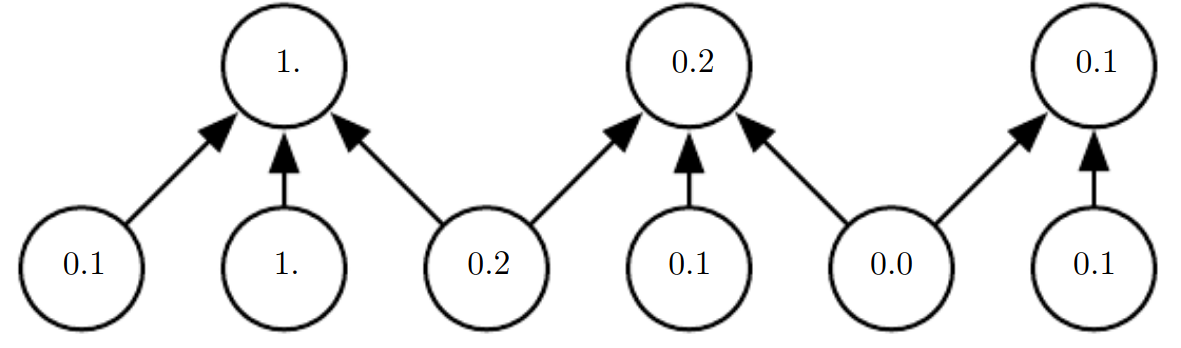
\includegraphics[width=1.0\textwidth]{maxpooling.png}
\caption{Primer združevanja s korakom $k=2$ in širino okna $3$. \cite{Goodfellow-et-al-2016}}
\end{figure}


\section{Rekurentne nevronske mreže}
\label{sec:nn:rnn}

Rekurentne nevronske mreže (RNN) so družina nevronskih mrež, ki se uporablja za obdelavo podatkov v zaporedjih. Prednost rekurentnih nevronskih mrež, pomembna za obdelavo zaporedij, je v tem da lahko hrani informacijo dlje časa. Zaradi te lastnosti lahko obdeluje daljša zaporedje, kot bi bilo praktično pri običajnih nevronskih mrežah. Večina rekurentnih nevronskih mrež lahko obdeluje podatke v zaporedjih različnih dolžin.

V primeru, da bi se obdelave zaporedij lotili z običajnimi nevronskimi mrežami, bi uporabili pristop z drsečim kontekstnim oknom določene širine. Slabost takšnega pristopa je omejen kontekst za zajem informacij, saj pojavnice zunaj kontekstnega okna na odločitve modela nimajo vpliva. Ta slabost je še izrazitejša pri jezikih, kjer so med seboj odvisne besede na različnih koncih povedi. Druga slabost je, da se model težje nauči vzorcev kot so besedne zveze.

Rekurentna nevronska mreža je vsaka nevronska mreža, ki vsebuje usmerjen cikel. V primeru ciklične povezave je enota posredno ali neposredno povezana s svojim izhodom na svoj vhod. Vrednost aktivacije rekurentne enote pri nekem koraku ni odvisna samo od vhoda, ampak tudi od vrednosti aktivacije v prejšnjem koraku. Rekurentne povezave omogočajo modeliranje časovne komponente zaporedij.

Obdelava niza podatkov z mrežami RNN poteka tako, da se elemente niza po vrsti vstavlja v mrežo. Rekurentna povezava daje način pomnjenja z uvajanjem informacije iz prejšnjega koraka. Takšna arhitektura ni omejena samo na prejšnji korak, saj vsi predhodni koraki vplivajo na trenutno stanje.

Glavna razlika med navadnimi nevronskimi mrežami in mrežami RNN je v dodatnih povezavah med skritim slojem v trenutnem korakom in skritim slojem prejšnjega koraka. Te povezave imajo tudi svoje uteži. Kot pri običajnih utežeh, se tudi uteži povezav med skritimi sloji učijo z vzvratnim razširjanjem napak.

\subsection*{Pojemajoči gradient}
Pojemajoči gradient je težava, ki se pojavlja pri učenju nevronskih mrež z gradientnimi metodami in vzvratnim razširjanjem napak. Pri gradientnih metodah dobijo uteži na vsakem koraku učenja nove vrednosti, ki so sorazmerne parcialnemu odvodu funkcije napake v odvisnosti od stare vrednosti uteži. Težava se pojavi, ko se gradient tako zmanjša, da postanejo spremembe vrednosti uteži neznatne. Uporaba aktivacijskih funkcij, pri katerih se pojavljajo odvodi z višjimi vrednostmi, lahko pripelje do obratnega problema, pri katerem gradient narašča prehitro.


\subsection*{Nevronske mreže LSTM}
Tipično se pri rekurentnih nevronskih mrežah informacija zakodirana v skritih stanjih najbolj navezuje na zadnji viden del vhodnega niza. Iz tega razloga se pri nalogah, ki zahtevajo uporabo informacij oddaljenih od trenutnega mesta obdelave pojavljajo težave. Pri obdelavi naravnega jezika, se pogosto pojavi potreba po poznavanju daljšega konteksta. Primer, ki se navezuje na temo pričujočega dela so odvisnosti med besedami, ki se nahajajo na različnih koncih dolge povedi.

Eden izmed razlogov za nezmožnost prenosa pomembne informacije je v tem, da sloj v rekurentni nevronski mreži opravlja dve nalogi hkrati. Prva naloga je priprava informacije, ki je koristna v trenutnem kontekstu. Druga naloga sloja pa je posodobitev in prenos informacije naprej, da je uporabna v prihodnjem kontekstu.

Druga težava, ki jo imajo rekurentne nevronske mreže pri učenju, je problem pojemajočega gradienta. Ta problem postene z daljšimi vhodnimi nizi še bolj izrazit.

Z namenom omejevanja teh težav so bili razviti pristopi, ki omogočajo ohranjanje informacije v daljših časovno odvisnih nizih. Ti pristopi obravnavajo kontekst spominsko enoto, ki jo je potrebno upravljati. Spominsko enoto se pri teh pristopih navadno upravlja s pozabljanjem in pomnjenjem.

Nevronske mreže z dolgim kratkoročnim spominom (Long short-term memory, LSTM), razpolagajo s kontekstom z optimizacijo dveh nalog. Prva je pomnjenje informacij, za katere je verjetno, da bodo pomembne pri prihodnjih odločitvah. Druga naloga pa je pozabljanje informacij, ki niso več potrebne. Nadzorovanje konteksta ni zakodirano v nevronske mreže LSTM, ampak se tega naučijo same.

Nevronske mreže LSTM imajo poleg zunanje rekurentnosti, ki je značilna tudi za navadne mreže RNN, tudi notranjo rekurentnost. Na zunaj je enota mreže LSTM ista kot enota navadne mreže RNN, saj ima iste vhode in izhode. V svoji notranjosti ima dodatno kompleksnost, zaradi česar ima tudi več parametrov. Notranja enota stanja ima linearno povezavo na sebe, zaradi katere se pojavi spominski učinek. Utež omenjene rekurentne povezave nadzirajo vrata, ki jim pravimo vrata pozabe. Vrata pozabe nadzirajo količino informacij, ki se na vsakem koraku ohrani. Na vhodu so še vhodna vrata, ki nadzirajo količino informacij, ki v trenutnem koraku vstopijo v celico in preprečujejo pomnjenje nepomembnih informacij. Izhodna vrata, na izhodu celice skrbijo za nadzor količine informacij ki se prenesejo v naslednji korak.


\label{sec:nn:lstm}

\section{Hitrocestne nevronske mreže}
\label{highway}

Družino nevronskih mrež, ki jo zaznamuje uporaba vrat za nadzor pretoka informacij skozi model in omogoča uporabo velikega števila slojev imenujem hitrocestne nevronske mreže \cite{Srivastava2015}.

Dejavnik, ki ključno vpliva na moč nevronske mreže je globina modela. Globina pomeni število slojev v nevronski mreži. Večja globina modelov je povezana z boljšo sposobnostjo aproksimacije določenih vrst funkcij.

Težava, ki se začne pojavljati z dodajnajem večjega števila slojev je oslabljeno razširjanje aktivacij in gradientov. Pristopi s katerimi se ta problem rešuje vključujejo boljše optimizacijske algoritme in nastavljanje začetnih uteži.

Drugačen pristop k povečanju števila slojev nevronske mreže brez omenjenih slabosti so hitrocestne nevronske mreže. Ta družina nevronskih mrež uporablja mehanizem vrat za nadzor pretoka informacij skozi enote. Takšen mehanizem omogoča tvorbo poti skozi katere lahko informacija potuje skozi več slojev brez slabljenja. Te poti se imenujejo hitre ceste.

Prednost takšnega pristopa je v tem, da ob velikemu številu slojev omogoča optimizacijo s stohastičnim gradientnim spustom (SGD), za razliko od navadnih nevronskih mrež, kjer ob velikem številu slojev SGD deluje slabo.

Avtorji članka Highway Networks \cite{Srivastava2015} so v svojih eksperimentih uporabili SGD na hitrocestnih nevronskih mrežah do globine 900 slojev. V primerjavi z običajnimi tesno povezanimi nevronskimi mrežami so pokazali, da se slednje tudi ob izboljšavi z normalizirano inicializacijo uteži opazno slabijo, medtem ko na hitrocestne mreže globina ne vpliva.

Pri običajni nevronski mreži lahko izhode nekega sloja opišemo z enačbo \ref{eq:highway1}, v kateri je $y$ vektor izhodov sloja, $x$ vektor vhodov, $H$ je nelinearna preslikava, $W_H$ pa so parametri preslikave $H$.

\begin{equation}
\label{eq:highway1}
y=H(x, W_H)
\end{equation}

$H$ je navadno afina preslikava, ki ji sledi nelinearna aktivacijska funkcija.

Sloji v hitrocestni nevronski mreži uvedejo še dve nelinearni preslikavi $T(x, W_T)$ in $C(x, W_C)$:

\begin{equation}
\label{eq:highway2}
y=H(x, W_H) \cdot T(x, W_T) + x \cdot C(x,W_C)
\end{equation}

Preslikavo $T$ imenujemo vrata preslikave, $C$ pa vrata prenosa. Poimenovanje izhaja iz dejstva, da ta vrata uravnavajo delež informacije, ki se nelinearno preslika in delež, ki je prenešen naprej.

\section{Rešitve sorodnih problemov z uporabo nevronskih mrež}
\label{sec:nn:solutions}

V preostanku poglavja predstavimo nekatere prispevke s področja modeliranja naravnega jezika z globokimi nevronskimi mrežami. Nekatere od rešitev namesto predstavitev besedila na nivoju besed uporabljajo predstavitve na nivoju znakov, ali pa združujejo oba pristopa. Glavni prednosti pristopa s predstavitvijo besedila na nivoju znakov sta:
\begin{description}
\item[Preprostejša priprava podatkov.] Edini vhodni podatki v takšen nevronski model so povedi, ki jih model vidi kot zaporedja znakov. Ta podatek dobimo neposredno iz jezikovnega korpusa in ne zahteva dodatne obdelave. Sorodne rešitve vpeljujejo dodatne značilke, ki jih tvorijo iz delov besed in besednih zvez ali pa jih vzamejo iz zunanjih virov, kot so leksikoni.
\item[Možnost boljših predstavitev podatkov.] Model predstavljen v \cite{Kim2015} lahko razdelimo na dva glavna dela. Jezikovni model, implementiran z rekurentnimi nevronskimi mrežami, je del, ki se iz vzorcev uči zakonitosti jezika. Drugi del, implementiran s konvolucijskimi nevronskimi mrežami, se uči vhodne podatke pretvoriti v jezikovnemu modelu uporabne vektorje značilk. Zasnova predstavitvenega modela je takšna, da spodbuja prepoznavo vzorcev kot so pogoste končnice in predpone besed ter druga pogosta zaporedja znakov.
\end{description}

\subsection*{Collobert, Weston, Bottou, Karlen, Kavukcuoglu, Kuksa (2011)\cite{Collobert2011}}
Avtorji predstavijo nevronsko mrežo z arhitekturo, ki je uporabna pri označevanju različnih zaporedij s področja obdelave naravnega jezika. Te naloge vključujejo oblikoskladenjsko označevanje, prepoznavo imenskih entitet in določanje semantičnih vlog.

To vsestransko uporabnost modela so dosegli s tem, da niso ročno tvorili značilk namenjenih točno določenim nalogam, ampak so pripravili model, ki se sam nauči iz besedila izluščiti uporabne lastnosti.

Model, ki so ga implementirali, ima na vhodu konvolucijski sloj, ki mu sledi združevalni sloj, nazadnje pa še več tesno povezanih slojev. Njihova nevronska mreža deluje na nivoju besed, ki vstopajo v model kot vektorske vložitve. Model so učili na korpusu, ki so ga zgradili iz celotne angleške Wikipedije in na korpusu Reuters RCV1 REF.

Svoj cilj, da bi razvili večnamenski model za različne vrste označevanja besedil so uresničili, saj so ocene njihovega označevalnika le rahlo zaostajale za ocenami najboljših, namenskih označevalikov.


\subsection*{Dos Santos, Zadrozny (2014)\cite{Santos2014}}
\label{nn:santos}
V tem članku je predstavljen model oblikoskladenjskega označevalnika z globokimi nevronskimi mrežami, ki združuje predstavitve na nivoju besed in na nivoju znakov. Globoka nevronska mreža, ki so jo zgradili ima na vhodu konvolucijski sloj, ki omogoča iskanje značilk iz besed poljubne dolžine. Tekom označevanja konvolucijski sloj gradi vektorske vložitve na nivoju znakov za vsako besedo, tudi za takšne, ki jih še ni videl v učni množici. Prednost pristopa k obdelavi besedila na nivoju znakov je v tem, da ni potrebno vnašati značilk s podatki o besedah in njihovih lastnosti.

Za demonstracijo učinkovitosti takšnega pristopa so razvili označevalnika za portugalski in angleški jezik. Oba označevalnika delujeta brez vpeljave dodatnih značilk. Angleški je dosegel 97,32\% točnost, portugalski pa 97,42\%.

V članku pokažejo tudi, da je za doseganje primerljivih rezultatov brez uporabe vložitev na nivoju znakov potrebno vpeljati dodatne, ročno pripravljene značilke. Kot slabost pristopa brez uvajanja dodatnih značilk navajajo dejstvo, da je pri takšnem modelu potrebno nastaviti več parametrov modela, kar pa po njihovem zahteva manj ročnega dela kot tvorjenje značilk.


\subsection*{Labeau, Allauzen (2016)\cite{Labeau2015}}
\label{nn:labeau}
Avtorji članka so uporabili različne arhitekture nevronskih mrež za implementacijo oblikoskladenskega označevalnika, ki deluje na nivoju znakov.

Deluje na dveh nivojih modeliranja, ki se učita hkrati. Ta nivoja sta konvolucijska nevronska mreža in tesno povezan nivo za napovedovanje oznak.

Konvolucijska nevronska mreža se uči predstavitev posameznih besed na nivoju znakov, napovedni nivoji pa se učijo iz teh predstavitev izpeljevati oblikoskladenjske oznake. Napovedni nivo so implementirali z uporabo tesno povezanih nevronskih mrež in z dvosmerno rekurentno mrežo. Model so učili na nemškem korpusu TIGER Treebank in svoje rezultate primerjali z označevalnikom ki temelji na algoritmu CRF (REF Mueller et al., 2013). V primerjavi rezultatov so pokazali, da njihov model na nivoju znakov vedno deluje bolje kot njihova implementacija nevronskega označevalnika na nivoju besed. Najboljšim rezultatom označevalnika z algoritmom CRF se je najbolj približal model, ki združuje predstavitvi na nivoju znakov in na nivoju besed.


\subsection*{Kim, Jernite, Sontag, Rush (2015) \cite{Kim2015}}
Avtorji predstavijo jezikovni model osnovan na globokih nevronskih mrežah. Kot pri zgornjih dveh rešitvah (\ref{nn:santos}, \ref{nn:labeau}), je bil tudi tukaj uporabljen pristop z vhodi na nivoju znakov in ne na nivoju besed, oziroma pojavnic, kot je to pri jezikovnih modelih običajno. 

Njihov jezikovni model je opravljal nalogo napovedovanja naslednje besede. Struktura nevronske mreže je podobna prejšnjim rešitvam opisanim v tem podpoglavju. Zgradba modela s primerom uporabe je vidna na sliki \ref{fig:kimmodel}. V svojem modelu so uporabil tudi hitrocestno nevronsko mrežo med konvolucijskimi in rekurentnimi sloji. V primerjavi rezultatov so opazili, da njihov jezikovni model ob uporabi hitrocestne mreže daje boljšo oceno čudenja, kakor model, ki vmesne hitrocestne mreže ne uporablja.

\begin{figure}
\label{fig:kimmodel}
\centering

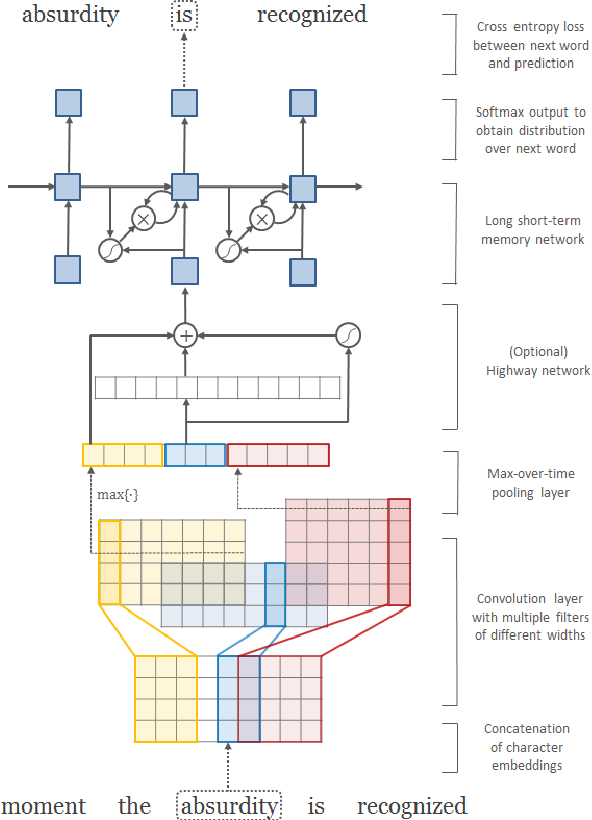
\includegraphics[width=0.8\textwidth]{kimmodel.png}
\caption{Arhitektura modela za napovedovanje naslednje besede z vhodi na nivoju znakov. Takšen jezikovni model je bil predstavljen v \cite{Kim2015}. Vhod na nivoju znakov je na spodnji strani skice. Od spodaj navzgor vhodu sledijo preslikave v vektorske vložitve znakov, konvolucijski filtri različnih širin, združevalni sloji s časovnim maksimumom, hitrocestna nevronska mreža, mreža LSTM, in izhodni sloj enot z aktivacijo softmax.}
\end{figure}

%----------------------------------------------------------------
% Poglavje (Chapter) 4
%----------------------------------------------------------------
\chapter{Arhitektura rešitve}
\label{ch:arhitektura}

% Uvod: model iz kim et al (opisano že v poglavju 3)
% Priprava podatkov
V tem poglavju predstavimo zasnovo in implementacijo naše rešitve. Pri zasnovi rešitve zastavljenega problema smo se zgledovali po jezikovnem modelu predstavljenem v \cite{Kim2015}. Omenjeno rešitev smo vzeli za zgled, ker zadostuje našemu cilju, da bi se model nauči dodeljevati pravilne oznake, brez uvajanja dodatnih značilk, kot v \cite{Grcar2012} in \cite{Ljubesic2016}.

Glavni deli naše rešitve so priprava podatkov, zgradba označevalnika z nevronskimi mrežami. Za izboljšavo kvalitete napovedi našega označevalnika smo nazadnje implementirali še preprost ansambel, ki združuje naš označevalnik skupaj z označevalnikoma Obeliks \cite{Grcar2012} in Reldi \cite{Ljubesic2016}.

% Namen: zbrati podatke; preslikati v vektorje; zgraditi model ()
\section{Priprava podatkov}
Naš model smo učili na podatkih iz jezikovnega korpusa ssj500k, različice 2.0 \cite{ssj500kv2}. V času nastajanja pričujočega dela je bil to največji ročno označen korpus za slovenski jezik. Vključuje 586248 pojavnic v 27829 povedih, vsaki pojavnici pa je prirejena tudi oblikoskladenjska oznaka pa specifikacijah MULTEXT East REF.

Korpus je na voljo v dveh formatih: XML-TEI in vert. Format XML-TEI boljše predstavlja hierarhijo korpusa, prednost formata vert pa je, da je enostavnejši za razčlenjevanje. Korpus v formatu vert je besedilna zbirka, v kateri ima vsaka vrstica pojavnico skupaj s pripadajočimi oznakami. Vrednosti v vrstici so med sabo ločene s tabulatorjem. Ker smo iz korpusa potrebovali samo pare pojavnic in njihovih oznak, smo se odločili za format vert.

% (kratek) opis formata vert. Podrobnejše lahko korpus opišeš v poglavju 2.2
\subsection*{Izbor povedi}
Pri zgradbi nevronske mreže našega označevalnika smo se morali odločiti za določeno dolžino vhodnih povedi in pojavnic, ki jih bo naš model dovoljeval. Ta zahteva izhaja iz dejstva, da morajo imeti vhodni primeri v model enotne dimenzije.

Z večanjem dimenzij vhodnih podatkov narašča zahtevnost problema, s tem pa tudi čas učenja nevronskega modela. Iz tega razloga nismo želeli določiti našemu modelu prevelikih vhodnih dimenzij. Po drugi strani smo želeli ohraniti kar se da veliko primerov iz korpusa. Za lažji izbor omejitev dolžin, smo preverili porazdelitvi dolžin povedi in pojavnic. Porazdelitvi sta prikazani na slikah \ref{fig:dolzinepojavnic} in \ref{fig:dolzinepovedi}.

\begin{figure}[H]
\label{fig:dolzinepovedi}
\centering
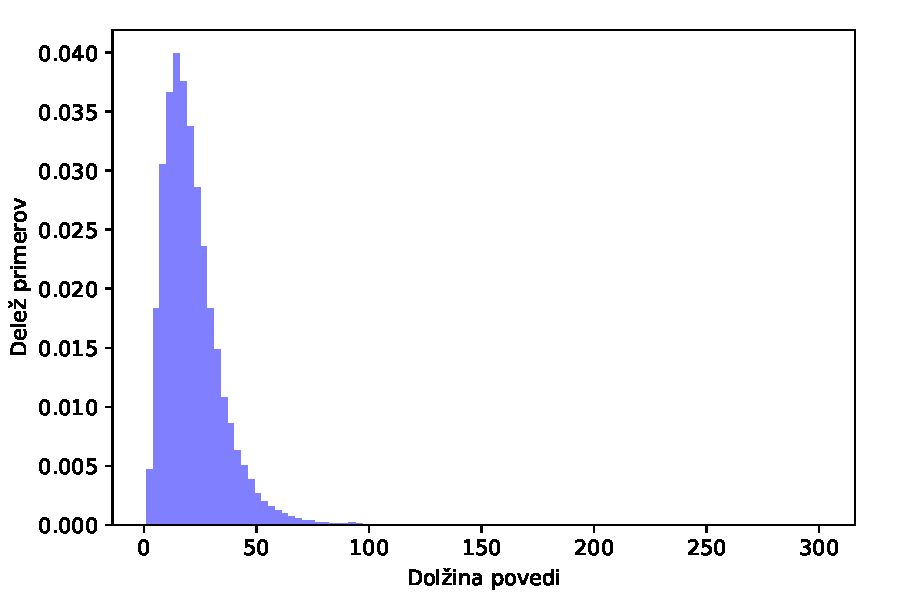
\includegraphics[width=0.7\textwidth]{len_povedi_hist.pdf}
\caption{Porazdelitev dolžin povedi v korpusu ssj500k. Dolžino povedi merimo s številom pojavnic.}
\end{figure}

\begin{figure}[H]
\label{fig:dolzinepojavnic}
\centering
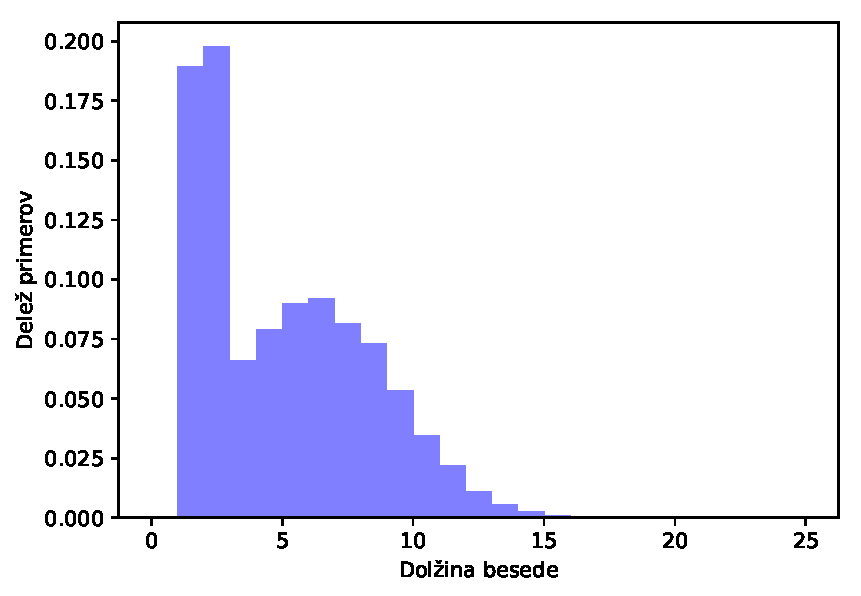
\includegraphics[width=0.7\textwidth]{len_besede_hist.pdf}
\caption{Porazdelitev dolžin pojavnic v korpusu ssj500k.}
\end{figure}

Za zgornjo mejo dolžin pojavnic smo izbrali dolžino dvajset znakov, za povedi pa 80 pojavnic. Po odstranitvi predolgih povedi iz korpusa, jih je od začetnih 27829 ostalo še 27702. Tako smo odstranili manj kot pol odstotka vseh primerov iz korpusa in si s tem omogočili omejitev dimenzionalnost vhodnih podatkov na spremenljivo velikost.


\subsection*{Pretvorba povedi v vektorske vložitve}

Podatke smo za obdelavo v nevronskem modelu pretvorili v vektorsko obliko. Vsako poved je bilo potrebno pretvoriti v matriko z dimenzijami, ki ustrezajo izbranim omejitvam dolžine. Ker smo povedi omejili na dolžino 80 pojavnic in pojavnice na 20 znakov, smo na tem koraku povedi pretvorili v matrike z 80 vrsticami in 20 stolpci.

Vrednosti v matriki smo zapolnili z indeksi znakov, prazna mesta pa zapolnili z ničlami. Spodnji primer ponazarja preslikavo povedi "To bi bila pravična vojna." v ustrezno matriko.

Dana poved je zaporedje pojavnic:
$$
\begin{pmatrix}
\text{To} \\
\text{bi} \\
\text{bila} \\
\text{pravična} \\
\text{vojna} \\
\text{.}
\end{pmatrix}
$$

Vsaki pojavnici preslikamo znake v indekse in jih vstavimo v vektor dolžine 20. Vektorje pojavnic zložimo skupaj v vektor povedi:

$$
\bordermatrix{
~      & 1  & 2  & 3 & 4 & 5 & 6 & 7 & 8 & 9 & \dots & 20 \cr
1      & 51 & 75 & 0  & 0  & 0 & 0 & 0 & 0 & 0 & \dots & 0 \cr
2      & 62 & 69 & 0  & 0  & 0 & 0 & 0 & 0 & 0 & \dots & 0 \cr
3      & 62 & 69 & 72 & 61 & 0 & 0 & 0 & 0 & 0 & \dots & 0 \cr
4      & 76 & 78 & 61 & 82 & 69 & 122 & 74 & 61 & 0 & \dots & 0\cr
5      & 82 & 75 & 70 & 74 & 61 & 0 & 0 & 0 & 0 & \dots & 0 \cr
6      & 14 & 0  & 0  & 0  & 0 & 0 & 0 & 0 & 0 & \dots & 0 \cr
7      & 0 & 0 & 0  & 0  & 0 & 0 & 0 & 0 & 0 & \dots & 0 \cr
\vdots & \vdots & \vdots & \vdots & \vdots & \vdots & \vdots & \vdots & \vdots & \vdots & \dots & \vdots \cr
80      & 0 & 0 & 0  & 0  & 0 & 0 & 0 & 0 & 0 & \dots & 0 \cr}
$$


\subsection*{Pretvorba oblikoskladenjskih oznak v vektorske vložitve}
Oblikoskladenjske oznake smo za ustrezno predstavitev v računalniškem pomnilniku preslikali v vektorske vložitve.

Pri tipičnem pristopu s področja strojnega učenja bi oznake predstavili s kodiranjem one-hot. Takšno
kodiranje ima v našem primeru dve pomanjkljivosti:
\begin{description}
\item[Velika prostorska zahtevnost] Vseh možnih oznak po specifikaciji MULTEXT East je 1900. To pomeni, da bi morali vsaki izmed pol milijona pojavnic v korpusu prirediti 1900 dimenzionalni vektor.
\item[Izguba informacij o odvisnostih med oznakami] Pri kodiranju one-hot so vsi razredi med sabo linearno neodvisni in si zato ne morejo deliti nekaterih istih ponavljajočih lastnosti. V našem primeru so takšne lastnosti sklon, spol, število in podobne, ki se pojavljajo pri različnih besednih vrstah.
\end{description}

Zaradi navedenih pomanjkljivosti smo uvedli novo kodiranje oblikoskladenjskih oznak. To kodiranje tvori gostejše vektorske vložitve oznak in omogoča deljenje posameznih lastnosti med različnimi vrstami oznak.

Za potrebo implementacije kodiranja smo iz specifikacij oblikoskladenjskih oznak zbrali vse možne lastnosti in njihove vrednosti. Posamezne lastnosti smo s kodiranjem one-hot preslikali v vektorske vložitve in jih zaporedno zložili v daljši vektor. Seznam lastnosti oblikoskladenjskih oznak je skupaj z njihovimi mesti v vektorskih vložitvah prikazan v tabeli \ref{tbl:indeks_lastnosti_oznak}.

S takšnim kodiranjem smo vektorje oznak v primerjavi s kodiranjem one-hot dosegli zmanjšanje dolžin vektorjev iz 1900 na 118. Poleg zmanjšanja dimenzionalnosti smo dosegli tudi deljenje lastnosti med različnimi oznakami. Tako se lahko naš model o pogostih besednih lastnostih v slovenskem jeziku uči preko različnih besednih vrst.

\begin{table}
\caption{Lokacije lastnosti v vektorski vložitvi oznak.}
    \begin{center}
        \begin{tabular}{l l l}
\hline
Lastnost & Začetek & Konec \\ \hline
Besedna vrsta & 1 & 13 \\
Določnost & 14 & 16 \\
Naslonskost & 17 & 19 \\
Nikalnost & 20 & 22 \\
Glagolska oblika & 23 & 30 \\
Oseba & 31 & 35 \\
Sklon & 36 & 43 \\
Spol & 44 & 48 \\
Spol svojine & 49 & 53 \\
Število & 54 & 58 \\
Število svojine & 59 & 63 \\
Stopnja pridevnika & 64 & 67 \\
Glagolski vid & 68 & 72 \\
Vrsta glagola & 73 & 75 \\
Vrsta neuvrščene pojavnice & 76 & 83 \\
Vrsta pridevnika & 84 & 87 \\
Vrsta prislova & 88 & 90 \\
Vrsta samostalnika & 91 & 93 \\
Vrsta števnika & 94 & 98 \\
Vrsta veznika & 99 & 101 \\
Vrsta zaimka & 102 & 111 \\
Zapis števnika & 112 & 115 \\
Živost samostalnika & 116 & 118 \\
\hline
        \end{tabular}
    \end{center}
\label{tbl:indeks_lastnosti_oznak}
\end{table}

Takšna predstavitev spremeni pristop k problemu. V primeru, da bi razrede predstavili s kodiranjem one-hot, bi oblikoskladenjsko označevanje reševali z večrazredno klasifikacijo, kjer bi bila vsaka možna oznaka en razred. V našem primeru imamo drugačen cilj, saj ne dodeljujemo enega razreda, temveč več različnih oznak. Sprememba pristopa ima to slabost, da lahko model napoveduje kombinacije oblikoskladenjskih lastnosti, ki ne sodijo skupaj in tako tvori neveljavne oblikoskladenjske oznake. Primer neveljavne oznake je glagol, ki mu model pripiše sklon.

Ta problem smo poskusili omejiti s tem, da smo vse vektorje lastnosti razširili z dodatnim poljem ki označuje, da ta lastnost ni veljavna. S temi dodatnimi polji smo želeli nevronskemu modelu eksplicitno označiti, kdaj določena lastnost ni veljavna.


\section{Nevronske mreže}
Pri strukturi nevronskega modela smo se zgledovali po modelu predstavljenem v \cite{Kim2015}. Nevronsko mrežo smo zgradili iz več delov, ki so med sabo funkcionalno ločeni.

\subsection*{Uporabljena orodja}

Za implementacijo nevronske mreže smo uporabili odprtokodno knjižnico Keras za programski jezik Python. Knjižnica Keras nudi enoten vmesnik za delo z implementacijami nevronskih mrež Tensorflow, Theano in Microsoft cognitive toolkit.

Keras omogoča enostavno gradnjo različnih vrst nevronskih mrež. Nudi gradnike, in ovojnice za gradnike, ki se jih da preprosto povezati v modele. Kljub preprosti uporabi, uporabniku dopušča svobodo pri nastavljanju parametrov.


\subsection*{Vhod}
Za začetni sloj v nevronski model smo določili Kerasov gradnik Input. Ta gradnik iz vhodnih podatkov zgradi vektorske vložitve.

V našem primeru so vhodni podatki vektorji besed, dolžine 20 znakov. Po zgledu iz \cite{Kim2015} smo gradniku Input določili dimenzijo 60, kar pomeni, da se vsak znak preslika v gosto vektorsko vložitev dolžine 60. Sloj Input tako preslika vhodne vektorje besed v matrike dimenzije $20 \times 60$.

Kot alternativa gostim vektorskim vložitvam znakov, bi lahko znake predstavili z redkimi vektorji one-hot, vendar bi v tem primeru imeli opravka z matrikami besed dimenzije $20 \times 131$, saj je v korpusu 131 različnih znakov, mi pa smo v našem modelu želeli obravnavati vse znake.

\subsection*{Predstavitveni model}
Vhodnemu sloju, ki pripravi vektorske vložitve znakov sledi več vzporednih konvolucijskih slojev. V \cite{Kim2015} so preizkusili dve konfiguraciji konvolucijskih slojev, ki se razlikujeta v številu slojev in številu enot v slojih. Ker poročajo o boljših rezultatih pri uporabi konfiguracije z več parametri, smo si tudi mi izbrali takšno.

Konvolucijska nevronska mreža, ki smo jo implementirali ima sedem vzporednih slojev. Vsi sloji uporabljajo aktivacijsko funkcijo hiperbolični tangens, razlikujejo pa se v številu filtrov in njihovi širini. Uprabljena konfiguracija je predstavljena v tabeli \ref{tbl:konfiguracijacnn}.

\begin{table}
\caption{Parametri konvolucijskih slojev}
    \begin{center}
        \begin{tabular}{l l l l}
        \hline
Širina filtrov & Število filtrov & Aktivacijska funkcija & Dimenzija izhoda \\ \hline
1 & 50 & $tanh$ & $20 \times 50$ \\
2 & 100 & $tanh$ & $20 \times 100$ \\
3 & 150 & $tanh$ & $20 \times 150$ \\
4 & 200 & $tanh$ & $20 \times 200$ \\
5 & 200 & $tanh$ & $20 \times 200$ \\
6 & 200 & $tanh$ & $20 \times 200$ \\
7 & 200 & $tanh$ & $20 \times 200$ \\ \hline
        \end{tabular}
    \end{center}
\label{tbl:konfiguracijacnn}
\end{table}

Vsakemu izmed konvolucijskih slojev sledi sloj globalnega združevanja po maksimumu \ref{pooling}. V teh slojih se izhodi konvolucijskih slojev strnejo v gostejši zapis, saj združevalna funkcija podatke v vsaki časovni enoti povzame z njihovim maksimumom. Tako dobljene združitve zložimo v skupni vektor.

Združevalnim slojem sledi še hitrocestna nevronska mreža \ref{highway}, s katero omogočimo lažji pretok informacij.

Do sedaj opisane sloje smo ovili z ovojnico TimeDistributed, ki omogoči modeliranje časovno odvisnih podatkov. V našem primeru so časovne enote besede v povedi.


\subsection*{Jezikovni model}

Del implementacije naše rešitve, ki je najbolj prilagojen za učenje zakonitosti jezika je implementiran z rekurentnimi nevronskimi mrežami z dolgim kratkoročnim spominom LSTM. Kot pri večjem izmed modelov, ki sta predstavljena v \cite{Kim2015}, smo tudi mi sloju LSTM dodelili 650 enot.

Jezikovni model iz \cite{Kim2015} smo prilagodili tako, da nismo imeli dveh slojev LSTM za obdelavo besedila v eno smer, ampak smo uporabili dvosmerni pristop. Pri našem pristopu smo sloju, ki podatke obdeluje v smeri iz leve proti desni dodali še sloj, ki deluje v obratno smer. S tem smo želeli naš model spodbuditi k odkrivanju odvisnoti med besedami v obeh smereh.

Jezikovni model smo implementirali z gradnikoma LSTM in Bidirectional, ki sta sestavni del knjižnice Keras. 

\subsection*{Odločitveni model}
%

Za določanje oznak smo kot zadnji gradnik našega modela dodali sloj tesno povezanih enot. Teh enot je 118; toliko, kolikor je dolžina naših predstavitev oznak. Ker smo želeli v vsaki izmed enot dobiti oceno verjetnosti smo uporabili za aktivacijsko funkcijo uporabili logistično funkcijo.

\section{Učenje modela}

Našo nevronsko mrežo smo med razvojem učili na 90 odstotkih celotne učne množice. Za funkcijo izgube smo določili binarno prečno entropijo. Binarna prečna entropija je primerna funkcija izgube pri problemih klasifikacije z več oznakami. Ta funkcija je že implementirana v knjižnici Tensorflow in podprta v Kerasu.

Dokončno sestavljen označevalnik smo učili z optimizacijskim algoritmom Adam v 30 sprehodih skozi učno množico. Na sliki \ref{fig:loss} je prikazano gibanje vrednosti funkcije izgube med učenjem. Pojemajoče padanje nakazuje, da se je algoritem približal optimumu, kar smo tudi potrdili s preizkusi na testni množici in s prečnim preverjanjem.

\begin{figure}[H]
\label{fig:loss}
\centering
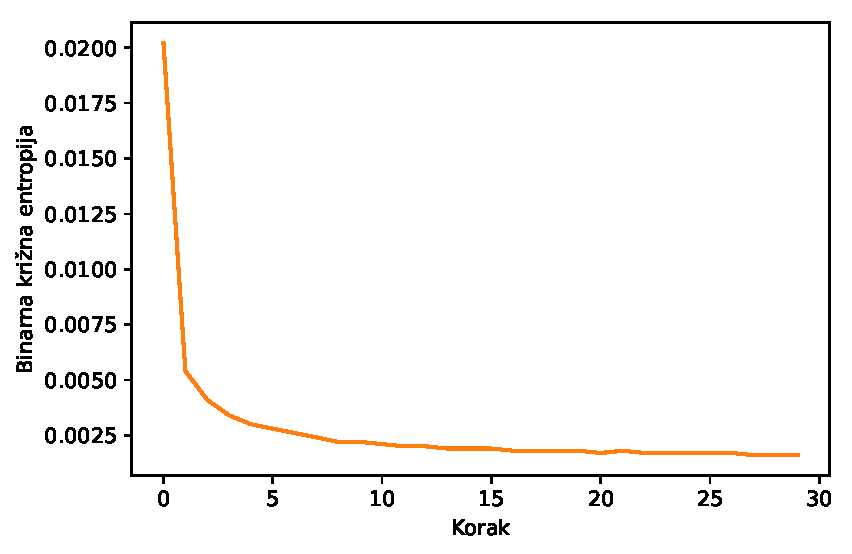
\includegraphics[width=1.0\textwidth]{loss.pdf}
\caption{Prikaz izgube pri učenju modela v 30 korakih.}
\end{figure}

\section{Ansambel označevalnikov}

Z namenom izboljšanja našega modela, smo implementirali preprost ansambel označevalnikov. V ansambel smo poleg naše rešitve vključili še označevalnika Obeliks \cite{Grcar2012} in Reldi \cite{Ljubesic2016}.

Implementirali smo preprost algoritem, ki oznake za vsako besedo vhodne povedi dodeljuje na podlagi glasovanja vključenih modelov. Algoritem v primeru treh različnih, veljavnih oznak vzame tisto, ki jo predlaga naš nevronski označevalnik. V primeru da nevronski označevalnik ustvari neveljavno kombinacijo oblikoskladenjskih lastnosti, algoritem vrne oznako, ki jo predlaga označevalnik Reldi. V ostalih primerih, ko vsaj dva označevalnika predlagata isto oznako, vrne algoritem predlog večine.

Pri implementaciji tega algoritma smo dali največjo težo našemu označevalniku, ker je v primerjavi označevalnikov dosegel najboljše ocene (podpoglavje \ref{rezultati}). Izjemo za primer neveljavnih oznak smo uvedli, ker naš označevalnik takšne oznake lahko tvori, za razliko od ostalih dveh označevalnikov, ki vedno vračata veljavne oznake.


%----------------------------------------------------------------
% Poglavje (Chapter) 5
%----------------------------------------------------------------
\chapter{Evalvacija}
\label{ch:evalvacija}
% * problem neobstoječih oznak
% Prečno preverjanje
\section{Primerjava označevalnikov}
\subsection*{Metodologija}

% točnost
% precision
% recall
% F1

% prečno preverjanje
\subsubsection*{Prečno preverjanje}

\subsection*{Rezultati}
\label{rezultati}

% za besedne vrste lahko razširjena ocena (f1, precision, recall)
% za celotne oznake samo klasifikacijska točnost
\begin{table}
\caption{ocene}
    \begin{center}
        \begin{tabular}{l l l}
        \hline
Označevalnik & Točnost besednih vrst & Točnost oznak \\ \hline
Obeliks & 0.923 & 0.810 \\
Reldi & 0.987 & 0.943 \\
Nevronski označevalnik & 0.988 & 0.956 \\
Ansambel z večino & 0.991 & 0.955 \\ \hline
        \end{tabular}
    \end{center}
\end{table}

\section{Analiza napak nevronskega označevalnika}


% matrike napačnih klasifikacij za posamezne dele oznak
% Rezultati
\begin{figure}
\centering
\caption{Matrika napačnih klasifikacij za besedne vrste. Izstopata razreda za medmet in neuvrščeno, ki ju model največkrat označi kot samostalnik.}
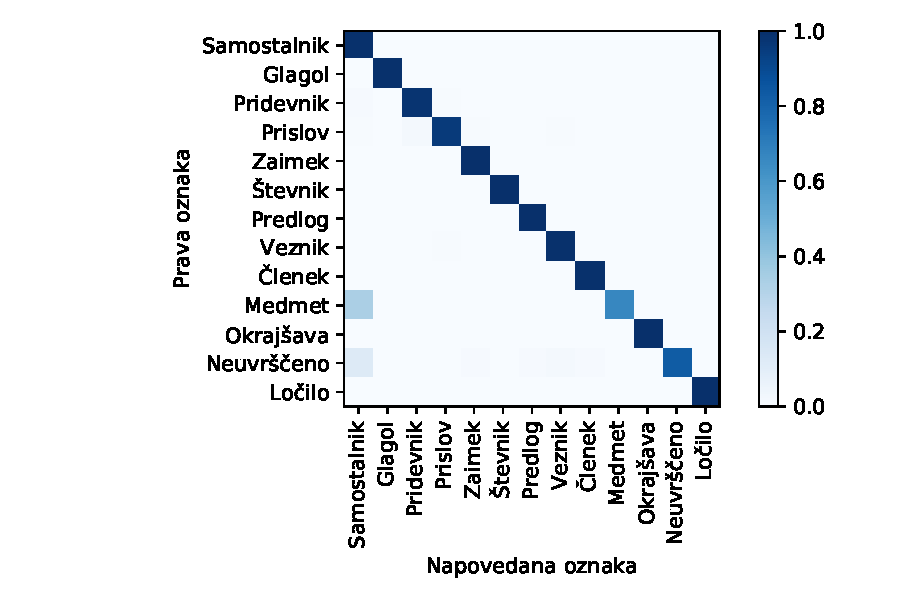
\includegraphics[width=1.0\textwidth]{besedne_vrste_norm.pdf}
\label{fig:confusionbv}
\end{figure}

\begin{figure}
\centering
\caption{Napačne klasifikacije za glagolsko obliko. Model največkrat napačno označi glagole v namenilniku in velelniku.}
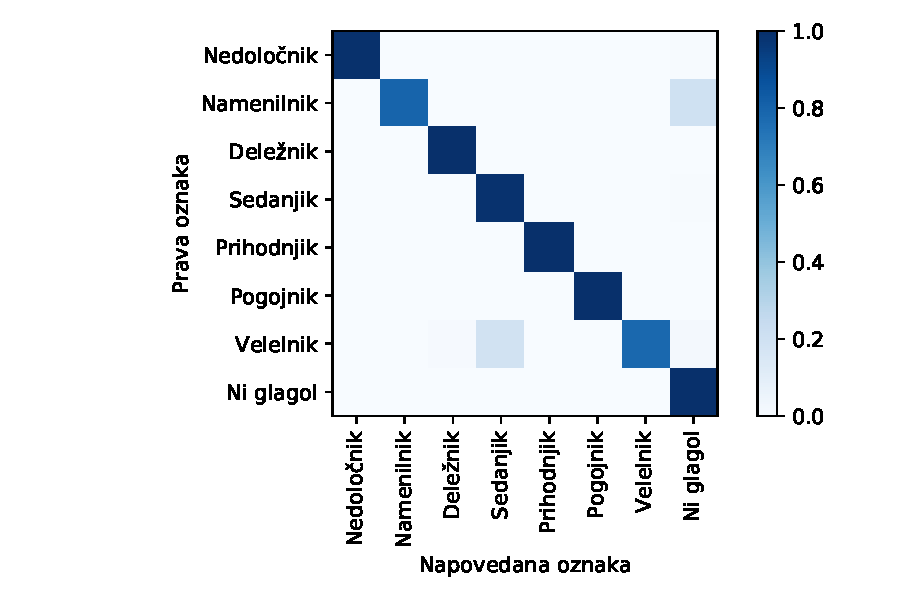
\includegraphics[width=1.0\textwidth]{glagolske_oblike_norm.pdf}
\label{fig:confusionglagolskeoblike}
\end{figure}

\begin{figure}
\centering
\caption{}
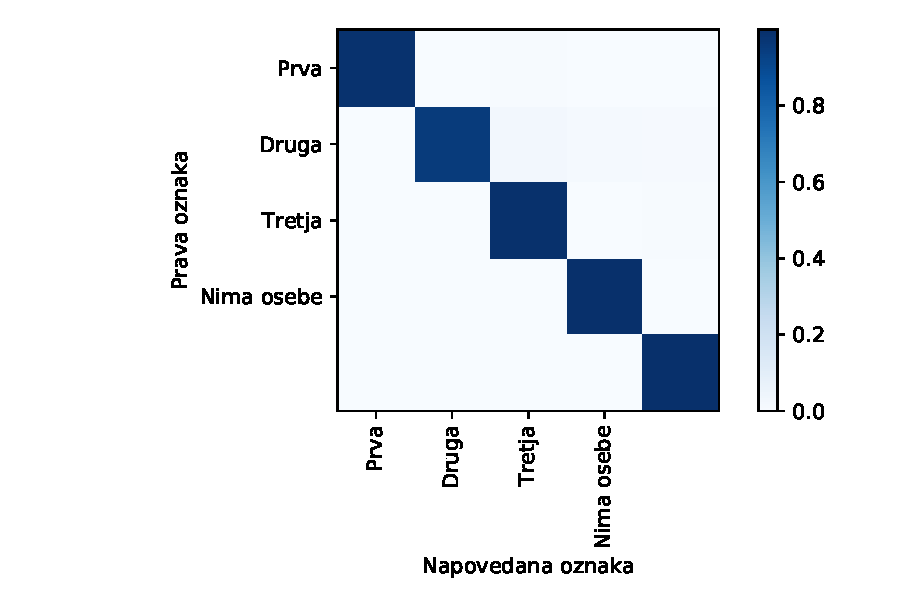
\includegraphics[width=1.0\textwidth]{osebe_norm.pdf}
\label{fig:confusionosebe}
\end{figure}

\begin{figure}
\centering
\caption{}
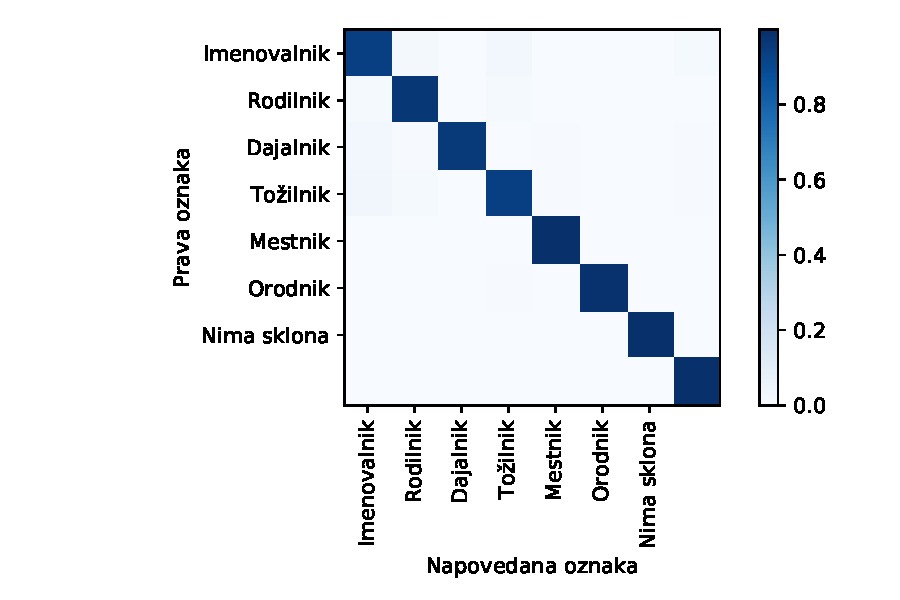
\includegraphics[width=1.0\textwidth]{skloni_norm.pdf}
\label{fig:confusionskloni}
\end{figure}


%----------------------------------------------------------------
% Poglavje (Chapter) 6
%----------------------------------------------------------------
\chapter{Zaključki}
\label{ch:zakljucki}

% * Problemi:
%   - neobstoječe oznake; kaznovanje takšnih oznak v loss funkciji
%   - vse možne oznake niso zastopane v naboru podatkov


%----------------------------------------------------------------
% SLO: bibliografija
% ENG: bibliography
%----------------------------------------------------------------
%\bibliographystyle{elsarticle-num}

%----------------------------------------------------------------
% SLO: odkomentiraj za uporabo zunanje datoteke .bib (ne pozabi je potem prevesti!)
% ENG: uncomment to use .bib file (don't forget to compile it!)
%----------------------------------------------------------------
%\bibliography{bibliography}

%----------------------------------------------------------------
% SLO: zakomentiraj spodnji del, če uporabljaš zunanjo .bib datoteko
% ENG: comment the part below if using the .bib file
%----------------------------------------------------------------

%\begin{thebibliography}{99}

%\bibitem{Fortnow} L.\ Fortnow, ``Viewpoint: Time for computer science to grow up'',
%{\it Communications of the ACM}, št.\ 52, zv.\ 8, str.\ 33--35, 2009.
%\bibitem{Knuth} D.\ E.\ Knuth, P. Bendix. ``Simple word problems in universal algebras'', v zborniku: Computational Problems in Abstract Algebra (ur. J. Leech), 1970, str. 263--297.
%\bibitem{Lamport} L.\ Lamport. {\it LaTEX: A Document Preparation System}. Addison-Wesley, 1986.
%\bibitem{ubi} O.\ Patashnik (1998) \BibTeX{}ing.
%Dostopno na: \url{http://ftp.univie.ac.at/packages/tex/biblio/bibtex/contrib/doc/btxdoc.pdf}
%\bibitem{licence} licence-cc.pdf. Dostopno na: \url{https://ucilnica.fri.uni-lj.si/course/view.php?id=274}
%\end{thebibliography}

\bibliographystyle{./bibliography/elsarticle-num}
\bibliography{./bibliography/bibliography}
\end{document}
